\documentclass[12pt]{report}
\usepackage[utf8]{inputenc}
\usepackage[export]{adjustbox}
\usepackage{amsmath,mathtools}
% \usepackage[subpreambles=true]{standalone}
\usepackage{ragged2e}
\usepackage[english]{babel}
\usepackage{siunitx}
% \usepackage{cite}
\usepackage{braket}
\usepackage{geometry}
\geometry{left = 2cm,right = 2cm,top = 4cm}

\usepackage{lipsum} % For dummy text
\usepackage{physics} % For physics notation
\usepackage{amssymb} % For math symbols 
\usepackage{gensymb} % For degree symbol
\usepackage{diagbox} % For table
\usepackage{hyperref}
\usepackage{xcolor} % for colored text
\usepackage{graphicx} % For \includegraphics
\usepackage{float}    % For the [H] placement specifier
% \usepackage{biblatex} %Imports biblatex package
\usepackage[
backend=biber,
style=alphabetic,
sorting=ynt
]{biblatex}
\usepackage{csquotes} % for biblatex
\addbibresource{bib.bib} %Import the bibliography file
\usepackage{rotating}
\usepackage{tabularx}
\usepackage{array}
% for code listing
\usepackage{listings}
\renewcommand{\lstlistingname}{Code}
\lstset{captionpos=b} % set the caption position to bottom
% \graphicspath{ {images/} }
\usepackage{datetime}
\usepackage{appendix}
\usepackage[stable]{footmisc} %for footnote in title
\usepackage{caption}

\title{

\includegraphics[width=0.25\textwidth]{nus_logo.jpeg}
\includegraphics[width=0.32\textwidth]{cqt_logo.png}\\
{\LARGE \textbf{
    Bosonic State Preparation Through Coupling With Semicon-spin Qubit Using Numerically Optimized Pulse Sequences
    }}\\
\vspace{5mm}
{Final Year Project Report}
}

\author{
    {\normalsize Lin Zhonglin \hspace{10mm} A0222183N}\\
    \vspace{1mm}
    {\normalsize Supervisor: Associate Professor Ng Huikhoon}\\
    {\normalsize Co-supervisor: Dr Koh Teck Seng}
}
\date{
    {\normalsize Department of Physics}\\
    {\normalsize National University of Singapore}\\
    {\normalsize Apr 2024}
}

\begin{document}
\justifying
\linespread{1.2}
\setlength{\parskip}{1em}
\setlength{\parindent}{0pt}

\maketitle


%%%%%%%%%%%%%%%%%%%%%%%%%%%%%%%%%%%%%%%%%%%%%%%%%%%%%%%%%%%%%%
\chapter*{Abstract}
Quantum computing leverages quantum mechanics principles, using qubits that can exist in multiple states simultaneously, enabling parallel processing. 
Various physical implementations such as superconducting qubits, trapped ions, and quantum dots have emerged as possible quantum computing platforms.
Besides traditional discrete quantum variable quantum computing where physical qubits represent logical qubits, an emerging continuous variable quantum computing uses usually infinite-dimensional quantum systems (like cavity states) to encode logical qubits, offering a different approach to error correction. \cite{RevModPhys.77.513}
One common platform for continuous variable quantum computing is cavity coupled to an auxiliary qubit for control.
This is often termed "bosonic qubits in circuit QED".\cite{Joshi_2021} In this area of quantum computing, the common physical platform is cavity coupled to a transmon. In this report we consider a possible alternative, cavity coupled to a Double Quantum Dot (DQD). \cite{D_Anjou_2019}
Moreover, in order to do quantum computation on a physical system, being able to do state preparation on the physical system is crucial, as it initializes qubits for computation, with prepared state fidelity impacting the overall performance of quantum algorithms. \cite{Nielsen2010}
In this report I focus on simultaneous control pulse optimization for state preparation of a cavity cat state on a cavity-DQD physical system (as opposed to driving cavity and qubit sequentially ). 
Pulse optimization for the overall composit state was successfully run for effective Hamiltonian (in restricted regime) of the system to arbitrarily high fidelity.
Though intended, optimization for the cavity state alone was not achieved; 
cheking the fidelity of the optimized pulses when run using the full physical Hamiltonian couldn't be attained in reasonable computation time;
optimization under noise was not achieved.  
Details on unreached goals and challenges faced can be seen in chapter \ref{sec:further_discussions}.

%%%%%%%%%%%%%%%%%%%%%%%%%%%%%%%%%%%%%%%%%%%%%%%%%%%%%%%%%%%%%%
\chapter*{Acknowledgements}
I would like to thank Associate Professor Ng Huikhoon and Dr Koh Tech Seng for this opportunity to gain invaluable experience in a quantum computation research group and also for their patience with me every Monday for the past eight months.
I would also like to thank seniors Siyan and Chiyuan who have given me incredible support and guidance as I struggled through the project that is in a field very new to me. 
I would also like to thank all the other seniors in Huikhoon's research group, especially Lukas who gave me many programming supports.
This project would not have been possible without the superb people mentioned.

\tableofcontents
%%%%%%%%%%%%%%%%%%%%%%%%%%%%%%%%%%%%%%%%%%%%%%%%%%%%%%%%%%%%%%
\chapter{Introduction}
%%%%%% 草稿 %%%%%%%%
% include: 
% - quantum computing background 
% -> continuous quantum computing 
% -> transmon-cavity 
% -> DQD-cavity 
% -> state preparation 
% -> pulse optimization 
% - Key part of my work

% 3-4 pages
% Introduction to quantum computing,
%   ->(1000 words)
%       - basics of quantum computing, its advantages over classical computing
%       - physical implementations of qubits, superconducting qubits, trapped ions, quantum dots
%       - motivate for continuous variable quantum computing, typical physical implementation of cavity-transmon implementation
%       - talk about the shortcomings of traditional cavity-transmon system, introduce the alternative cavity-DQD system, its advantages and potential
%       - state preparation in quantum computing, its importance and challenges -> need state preparation for passing into quantum gates, etc
%       - introduce pulse optimization as a method for state preparation, its importance and challenges
%   -> discuss my work: (300 words)
%       - methodology and overall plan
%       - obtained results
%       - tasks not completed and challenged causing these failure
%       - possible future work

% (reference each paragraph to the relaevant sections in the report)
%%%%%% 草稿 %%%%%%%%
Quantum computing has emerged as a paradigm with the potential to solve problems that are intractable for classical computers. 
By leveraging the principles of quantum mechanics, such as superposition and entanglement, quantum computers can perform certain computations exponentially faster than their classical counterparts \cite{Nielsen2010}. 
This has led to significant interest in developing practical quantum computing systems and algorithms for various applications, ranging from cryptography and optimization to quantum simulation and machine learning \cite{Preskill2018}.
\par
At the heart of quantum computing lies the qubit, the fundamental unit of quantum information. 
Unlike classical bits, which can only be in one of two states (0 or 1), qubits can exist in a superposition of multiple states simultaneously. 
This property, along with the ability to create entanglement between qubits, enables quantum computers to explore vast computational spaces in parallel \cite{Nielsen2010}. 
However, realizing robust and scalable qubits is a significant challenge due to their susceptibility to noise and decoherence.
\par
Various physical implementations of qubits have been proposed and experimentally demonstrated, each with its own advantages and limitations. 
Superconducting qubits, which utilize the collective behavior of cooper pairs in superconducting circuits, have emerged as a leading platform due to their strong nonlinearity, fast gate operations, and compatibility with existing microwave technology \cite{Kjaergaard2020}. 
Trapped ion qubits, on the other hand, leverage the electronic states of ions confined in electromagnetic traps, offering long coherence times and high-fidelity gate operations \cite{Bruzewicz2019}. 
Quantum dots, which are nanoscale structures that confine electrons or holes, have also shown promise as a scalable and easily controllable qubit platform \cite{Chatterjee2021}.
\par
In addition to the traditional approach of encoding qubits in discrete two-level systems, there has been growing interest in continuous variable quantum computing (CVQC). 
CVQC utilizes the infinite-dimensional Hilbert space of bosonic modes, such as those of electromagnetic fields or mechanical oscillators, to encode and process quantum information \cite{Braunstein2005}. 
Such a scheme is desirable because it enables more elaborate encoding that encodes a single logical qubit on multiple physical qubits while still requiring control of a single physical system.
One of the most prominent physical implementations of CVQC is the cavity-transmon system, where a superconducting transmon qubit is coupled to a microwave cavity. This hybrid approach combines the long coherence times of cavities with the strong nonlinearity and fast control of transmon qubits, enabling a range of quantum operations and error correction schemes \cite{Ofek2016}.
\par
However, the cavity-transmon system also has its limitations, such as its relatively short coherence times of transmon qubits compared to other platforms. 
An alternative approach is to couple the cavity to a double quantum dot (DQD) instead of a transmon. 
The cavity-DQD system has the potential to combine the advantages of semiconductor quantum dots, such as long coherence times and compatibility with existing semiconductor technology, with the benefits of CVQC \cite{Mi2018}. 
This hybrid platform opens up new possibilities for quantum information processing and provides a promising avenue for scalable quantum computing \cite{Burkard2020}. (chapter \ref{sec:physical_system})
\par
One of the key challenges in quantum computing is state preparation, which involves initializing the qubits in a desired quantum state before performing any computation. 
The state fidelity and efficiency of state preparation directly impact the overall performance of quantum algorithms and the reliability of quantum error correction schemes \cite{Shen2017}. 
In CVQC, state preparation often involves creating non-classical states, such as Schrödinger cat states or squeezed states, which are essential for various logical qubit encoding schemes \cite{Joshi_2021}. 
However, preparing these states with high fidelity is a non-trivial task due to the presence of noise and the limitations of control techniques.
\par
Pulse optimization has emerged as a powerful method for state preparation in quantum systems. 
By carefully designing the time-dependent control pulses applied to the qubits or cavities, one can steer the system towards the desired target state while minimizing the effects of noise and decoherence \cite{Khaneja2005}. 
Quantum optimal control theory provides a framework for finding the optimal control pulses that maximize the fidelity of state preparation or gate operations \cite{Glaser2015}. 
It has been shown by \cite{Krastanov2015} which gave a construction for how to achieve arbitrary operations on dispersively coupled cQED systems (which includes my system of interest) using a set of two operations: displacements and selective number-dependent arbitrary phase (SNAP) operations.
Hence, this project focuses on achieving cavity state preparation by first optimizing for selective qubit rotations (this report focuses on qubit flipping). 
My research group colleage Chiyuan has carried out a state preparation on the same physical system by first analytically solving then driving the caivty and qubit sequentially. 
Such an analytical is a good proof of concept. 
However, it is not necessarily the most gate time efficient approach when it comes to applying to actual physical state preparation as it is not utilizing the full optimization landscape, but only a special solution. 
Hence, this project which allows for simultaneous driving of the cavity and qubit serves as an extension of Chiyuan's work.
(chapter \ref{sec:methodology} and \ref{sec:state_preparation})
\par
In this project, we focus on exploring quantum optimal control techniques for state preparation in the cavity-DQD system. 
Our methodology involves first deriving the effective Hamiltonian that describes the dynamics of the coupled cavity-DQD system in the dispersive regime. 
We then formulate the state preparation problem as an optimization task, where the goal is to find the control pulses that maximize the fidelity between the evolved state and the target state. 
We employ various optimization algorithms, such as GRAPE (GRadient Ascent Pulse Engineering) and CRAB (Chopped RAndom Basis), to numerically search for the optimal pulses \cite{KHANEJA2005296, PhysRevLett.106.190501}. 
(chapter \ref{sec:methodology} and \ref{sec:state_preparation})
\par
Here is a summary of optimization results: 
\begin{sidewaystable}
    \begin{tabularx}{\textheight}{|p{4cm}|p{2cm}|X|X|p{2cm}|X|X|X|X|}
    \hline
    name                               & \begin{tabular}[c]{@{}l@{}}physical\\ system\end{tabular}             & \begin{tabular}[c]{@{}l@{}}initial\\ state\end{tabular} & \begin{tabular}[c]{@{}l@{}}target\\ state\end{tabular}  & \begin{tabular}[c]{@{}l@{}}ops\\ algo\end{tabular} & N(Fock space truncation)     & \begin{tabular}[c]{@{}l@{}} time \\ discre- \\ -tisation\end{tabular} & \begin{tabular}[c]{@{}l@{}}pulse\\ length \\ (ns) \end{tabular} & \begin{tabular}[c]{@{}l@{}}final\\ fidelity\\ (simulation)\end{tabular} \\ \hline
    single\_qubit                      & \begin{tabular}[c]{@{}l@{}}single\\ qubit\end{tabular}                & \begin{tabular}[c]{@{}l@{}}ground\\ state\end{tabular}  & \begin{tabular}[c]{@{}l@{}}excited\\ state\end{tabular} & GRAPE                                              & NIL & 1000                                                           & 18                                                     & 0.9999                                                      \\ \hline
    vaccuum2coherent                       & \begin{tabular}[c]{@{}l@{}}cavity\\ coupled to\\ a qubit\end{tabular} & $\psi_{i1}$                                             & $\psi_{f1}$                                             & GRAPE                                              & 5     & 100                                                            & 1                                                      & 0.9999                                                        \\ \hline
    unselective\_spin\_flip            & \begin{tabular}[c]{@{}l@{}}cavity\\ coupled to\\ a qubit\end{tabular} & $\psi_{i2}$                                                        & $\psi_{f2}$                                                       & GRAPE                                              & 16    & 500                                                            & 1                                                      & 0.9995                                                      \\ \hline
    selective\_spin\_flip              & \begin{tabular}[c]{@{}l@{}}cavity\\ coupled to\\ a qubit\end{tabular} & $\psi_{i3}$                                                        & $\psi_{f3}$                                                       & GRAPE                                              & 16    & 100000                                                         & 500                                                    & 0.9994                                                      \\ \hline
    \begin{tabular}[c]{@{}l@{}}selective\_spin\_flip\\ \_constraints\end{tabular} & \begin{tabular}[c]{@{}l@{}}cavity\\ coupled to\\ a qubit\end{tabular} & $\psi_{i3}$             & $\psi_{f3}$                                                        & GRAPE                                              & 16    & 100000                                                         & 500                                                    & 0.9992                                                      \\ \hline
    vacuum2cat                            & \begin{tabular}[c]{@{}l@{}}cavity\\ coupled to\\ a qubit\end{tabular} & $\psi_{i4}$                                                        & $\psi_{f4}$                                                        & GRAPE                                              & 16    & 100000                                                         & 5000                                                   & 0.9529                                                                        \\ \hline
    vacuum2cat                            & \begin{tabular}[c]{@{}l@{}}cavity\\ coupled to\\ a qubit\end{tabular} & $\psi_{i4}$                                                        & $\psi_{f4}$                                                        & KROTOV                                              & 16    & 100000                                                         & 5000                                                   & 0.9995                                                                       \\ \hline
    \end{tabularx}
\end{sidewaystable}

where, initial and target states are given by: 
\begin{align*}
    % vac2coherent
    \text{vac2coherent} \\
    \psi_{i1} &= \ket{0}_{\text{cavity}} \otimes \ket{0}_{\text{qubit}} \\
    \psi_{f1} &= \ket{\alpha}_{\text{cavity}} \otimes \ket{0}_{\text{qubit}} \\
    % unselective
    \text{unselective} \\
    \psi_{i2} &= \frac{1}{\sqrt{2}} (\ket{0}_{\text{cavity}} \otimes \ket{0}_{\text{qubit}} 
                + \ket{1}_{\text{cavity}} \otimes \ket{0}_{\text{qubit}})\\
    \psi_{f2} &= \frac{1}{\sqrt{2}} (\ket{0}_{\text{cavity}} \otimes \ket{1}_{\text{qubit}} 
                + \ket{1}_{\text{cavity}} \otimes \ket{1}_{\text{qubit}})\\
    % selective
    \text{selective} \\
    \psi_{i3} &= \frac{1}{\sqrt{2}} (\ket{0}_{\text{cavity}} \otimes \ket{0}_{\text{qubit}} 
                + \ket{1}_{\text{cavity}} \otimes \ket{0}_{\text{qubit}})\\
    \psi_{f3} &= \frac{1}{\sqrt{2}} (\ket{0}_{\text{cavity}} \otimes \ket{0}_{\text{qubit}} 
                + \ket{1}_{\text{cavity}} \otimes \ket{1}_{\text{qubit}})\\
    % vac2cat
    \text{vac2cat} \\
    \psi_{i1} &= \ket{0}_{\text{cavity}} \otimes \ket{0}_{\text{qubit}} \\
    \psi_{f1} &= \ket{\alpha}_{\text{cavity}} \otimes \ket{0}_{\text{qubit}} 
                + \ket{-\alpha}_{\text{cavity}} \otimes \ket{0}_{\text{qubit}} \\
\end{align*}

The project aimed to optimize control pulses for state preparation of a cavity vacuum state to cavity cat state in a cavity-coupled double quantum dot system.
The original goal was to first optimize for high state fidelity using an effective Hamiltonian of the system and make sure that the optimized pulses work well when using the original full Hamiltonian.
If this is to be achieved, other potential goals include optimization under physical pulse constraints, optimization for a open quantum system (considering noise), optimization for other state optimizations, optimization for gates.
However, several challenges were encountered that prevented reaching the initial goals within the given timeframe. Here I list the goals not achieved and outline the challenges faced.
Firstly, QuTip's implementation made it difficult to optimize the fidelity of the cavity state alone by partial tracing out the qubit state, requiring a significant rewrite of the optimization code. 
Although the Krotov package seems to allow for customization of fidelity, this was not attempted due to time constraints. 
Secondly, the project did not fully consider all physical constraints on the control pulses, with only pulse amplitude constraints being implemented. 
The CRAB algorithm could be used to incorporate more constraints and optimize functional basis coefficients for smoother pulses, but requires more trial and error. This was also not attempted due to time constraints.
Thirdly, the native oscillation frequency of the cavity caused fast oscillations in the optimized pulses, which could potentially be addressed but issues also came up. See chapter \ref{sec:further_discussions} for more details.
Though it was unfortunate that many of the original goals were not achieved due to time constraints, all of these challenges seem to be technical difficulties. 
With more time, these technical programming issues could be resolved.

%%%%%%%%%%%%%%%%%%%%%%%%%%%%%%%%%%%%%%%%%%%%%%%%%%%%%%%%%%%%%%
\chapter{Physical System and Hamiltonians: DQD-cavity}\label{sec:physical_system}
%%%%%% 草稿 %%%%%%%%
% discuss
% - Full Original Hamiltonian 
% - effective Hamiltonian 
% - link clearly the Hamiltonians here to the Hamiltonians used in the methodology chapter later
% main papers: 
% - Optimal dispersive readout of a spin qubit with a microwave resonator

%%%%%% 草稿 %%%%%%%%
% First to reiterate briefly on why we are interested in a cavity-DQD system. Strong coupling of semiconductor spin qubits to superconducting microwave resonators was recently demonstrated. \cite{Mi2018}\cite{Landig2018}
% These breakthroughs can potentially combine the long coherence times of solid-state spin qubits with the long-distance connectivity, fast control, and fast high-fidelity quantum-non-demolition readout of existing superconducting qubit implementations.\cite{D_Anjou_2019}
% Although this project doesn't reach the part of readout, but only considers state preparation in this physical system. This serves as a motivation. 
% The chapter below is adapted from \cite{D_Anjou_2019} and \cite{reinhold2019} as they explain the physical system and Hamiltonians very well. 
% This project focuses much more on optimization than on the physical systems themselves.
% \par
% We consider a DQD defined by a double-well potential $V(z)$ whose wells are separated by a distance $2d$, as depicted in Fig \ref{fig:DQD}.
% The two lowest-energy orbitals of the right and left wells are labelled $|\widetilde{R}\rangle$ and $|\widetilde{L}\rangle$, respectively, with corresponding energies $\epsilon_R$ and $\epsilon_L$.
% The energy detuning between the right and left orbitals is $\epsilon=\epsilon_R-\epsilon_L$, and the tunnel coupling between them is $t_c>0$. 
% Moreover, a uniform longitudinal magnetic field is applied along the axis of the quantum dot (the $z$ axis). This induces a Zeeman energy splitting $\hbar \gamma_e B_z$ of the electronic spin states $|\widetilde{\uparrow}\rangle$ and $|\widetilde{\downarrow}\rangle$, where $\gamma_e$ is the electron gyromagnetic ratio. 
% In addition, a transverse position-dependent magnetic field $B_x(z)$ is applied along the $x$ axis using, e.g., a proximal micromagnet. As the electron moves across the DQD, it therefore experiences a magnetic field variation of order $b_x=\partial_z B_x(z) \times d$. This hybridizes the spin and charge degrees of freedom, enabling electrical control and readout of the spin. 
% In the following, we set $\hbar=1$ and $\gamma_e=1$. The resulting DQD Hamiltonian is
% \begin{equation}\label{eq:DQD_Hamiltonian}
%     \begin{aligned} 
%         & H_d=H_m+H_Z, \\
%         & H_m=\frac{\epsilon}{2} \widetilde{\tau}_z+t_c \widetilde{\tau}_x, \\
%         & H_Z=\frac{B_z}{2} \widetilde{\sigma}_z+\frac{b_x}{2} \widetilde{\tau}_z \widetilde{\sigma}_x .
%     \end{aligned}    
% \end{equation}


% In Eq. \ref{eq:DQD_Hamiltonian}, $H_m$ is the molecular Hamiltonian of the DQD and $H_Z$ is the Zeeman Hamiltonian. Moreover, the $\widetilde{\tau}_i$ are the Pauli matrices in the $\{|\widetilde{R}\rangle,|\widetilde{L}\rangle\}$ basis and the $\widetilde{\sigma}_i$ are the Pauli matrices in the $\{|\widetilde{\uparrow}\rangle,|\widetilde{\downarrow}\rangle\}$ basis. 
% It is also convenient to introduce the eigenstates $|\widetilde{ \pm}\rangle$ of the molecular Hamiltonian $H_m$. They satisfy $H_m|\widetilde{\Psi}\rangle= \pm \frac{\Omega}{2}|\widetilde{\Psi}\rangle$, where $\Omega=\sqrt{\left(2 t_c\right)^2+\epsilon^2}=2 t_c \sec \theta$ is the molecular energy gap and where $\theta=\arctan \left(\epsilon / 2 t_c\right)$ is the molecular mixing angle. 
% Note that the description of electronic motion in terms of the two lowest-energy orbitals is only valid in the limit where $\Omega$ is much smaller than the single-dot orbital splitting, whether it originates from confinement or from valley splitting.
% \begin{figure}[H]
%     \centering
%     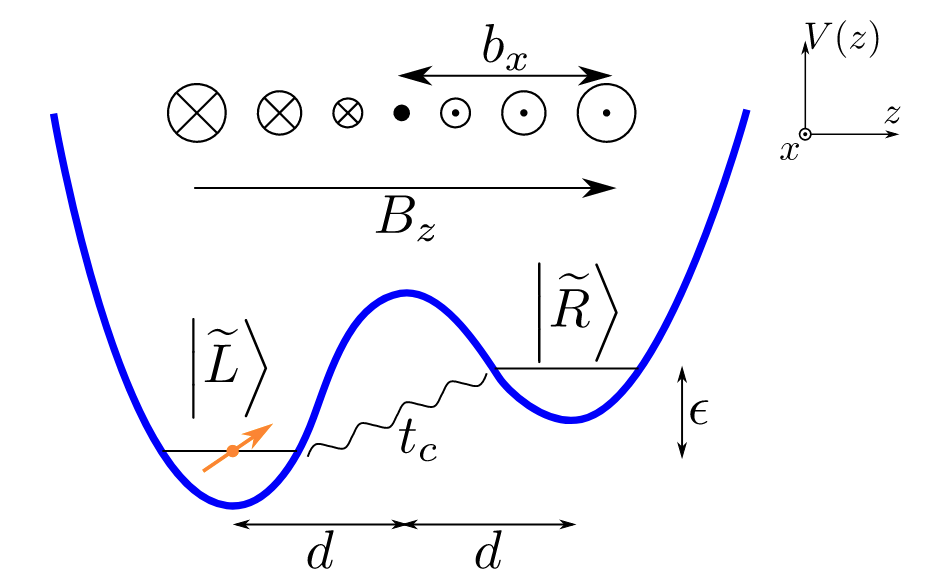
\includegraphics[width=0.5\linewidth]{DQD.png}
%     \caption{
%         (a) Schematic representation of the double-well potential $V(z)$ forming the DQD. The detuning and tunnel coupling between the right dot orbital $|\widetilde{R}\rangle$ and left dot orbital $|\widetilde{L}\rangle$ are $\epsilon$ and $t_c$, respectively. The DQD is subject to a longitudinal magnetic field $B_z \hat{z}$ and an external transverse magnetic field gradient $\partial_z B_x(z) \hat{x}$ such that the field $B_x$ varies by $b_x=\partial_z B_x(z) \times d$ over the half interdot distance $d$. (b) Setup for the dispersive readout of a DQD embedded in a two-port microwave resonator with resonance frequency $\omega_r$. The DQD and the resonator electric field (green arrows) interact via the electric dipole coupling $g_c$. The resonator can be driven in the $i$ th port by an input field $b_i^{\text {in }}(t)$. The output fields $b_i^{\text {out }}(t)$ then carry information on the state of the DQD. The leakage rates of ports 1 and 2 to their respective feedlines are $\kappa_1$ and $\kappa_2$.\cite{D_Anjou_2019}
%     }
%     \label{fig:DQD}
% \end{figure}

% % Double-quantum-dot-resonator interaction
% The electric field of the resonator couples directly to the electric dipole moment of the electron, as shown schematically in Fig. \ref{fig:DQD}(b). 
% Due to the interaction of the spin and orbit degrees of freedom, the resonator photons can drive spin transitions. 
% The Hamiltonian of the combined resonator and DQD system is
% \begin{equation}\label{eq:DQD_resonator_Hamiltonian}
%     \begin{aligned} 
%         & H=H_d+H_r+V, \\
%         & H_r=\omega_r a^{\dagger} a, \\    
%     & V=g_c \tilde{\tau}_z\left(a+a^{\dagger}\right) .
%     \end{aligned}
% \end{equation}

% In Eq. \ref{eq:DQD_resonator_Hamiltonian}, $H_r$ is the free Hamiltonian for a single mode of the resonator, $V$ is the dipole interaction Hamiltonian between the electron and the resonator, and $a$ annihilates a photon in the resonator. 
% The resonance frequency of the resonator is $\omega_r>0$ and the strength of the dipole coupling is $g_c$.

% % Double-quantum-dot eigenbasis and spin qubit
% The DQD Hamiltonian, Eq. (1), can be diagonalized exactly as detailed in cite{D_Anjou_2019} Appendix A. Expressed in its eigenbasis, the Hamiltonian $H_d$ takes the form
% \begin{equation}\label{eq:DQD_Hamiltonian_in_eigenbasis}
%     H_d=\frac{E_m}{2} \tau_z+\frac{E_s}{2} \sigma_z,    
% \end{equation}

% where the $\tau_i$ and the $\sigma_i$ are now Pauli matrices in the eigenbasis $\left|\tau_z ; \sigma_z\right\rangle$ of $H_d$ dressed by the field gradient. 
% Here $\tau_z= \pm$ labels the dressed "molecular-like" states and $\sigma_z=\uparrow(\downarrow)$ labels the dressed "spin-like" states [67]. 
% Exact expressions for the molecular-like and spin-like Larmour frequencies $E_m$ and $E_s$ are derived in \cite{D_Anjou_2019} Appendix A. The energy-level diagram of the DQD is illustrated in Fig. 2, where we have also introduced the transition frequencies $E_{ \pm}=E_m \pm E_s$. 
% In the following, we consider the spin qubit formed from the two dressed spin-like eigenstates spanning the molecular ground state. 
% Specifically, we choose the computational basis $\{|1\rangle,|0\rangle\}=$ $\{|-; \uparrow\rangle,|-; \downarrow\rangle\}$. 
% Despite their spin-like character, the electric dipole matrix element between these two states is finite and transitions between them can be induced electrically. 
% In particular, the DQD-resonator interaction of Eq. (2) is written in the new basis as
% \begin{equation}\label{eq:DQD_resonator_interaction_new_basis}
%     \begin{aligned}
%         V= & \mathcal{V}\left(a+a^{\dagger}\right), \\
%         \mathcal{V}= & -g_m \tau_x+g_s \tau_z \sigma_x+g_{+}\left(\tau_{+} \sigma_{+}+\tau_{-} \sigma_{-}\right) \\
%         & +g_{-}\left(\tau_{+} \sigma_{-}+\tau_{-} \sigma_{+}\right)+g_{m p} \tau_z+g_{s p} \sigma_z .
%         \end{aligned}    
% \end{equation}

% Here $\left\{g_m, g_s, g_{+}, g_{-}\right\}$are the coupling strengths of the resonator to the DQD transitions of frequencies $\left\{E_m, E_s, E_{+}, E_{-}\right\}$ illustrated in Fig. 2. 
% In addition, $g_{m p}$ and $g_{s p}$ are couplings arising from the finite dc electric polarizabilities of the molecular electric dipole and of the spin, respectively. 
% Exact expressions for the $g_i$ are given in \cite{D_Anjou_2019} Appendix A.
% \par
% The above chapter has been mostly lifted from \cite{D_Anjou_2019} for a detailed explaination of the original full Hamiltonian
% of the full Hamiltonian (as referenced later in chapter \ref{sec:further_discussions}).
% However, as discussed earlier this project focuses more on optimization using the effective Hamiltonian in the dispersive regime where the DQD is effectively a two-level system. 
% Derivation of the effective Hamiltonian is well written in \cite{reinhold2019} chapter 2.3, key formulas are reproduced here for later reference. 
% The model effective Hamiltonian is given by, 
% \begin{equation}\label{eq:effective_Hamiltonian}
%     \boldsymbol{H}=\omega_c \boldsymbol{a}^{\dagger} \boldsymbol{a}+\frac{\omega_q}{2} \boldsymbol{\sigma}_z+\frac{\chi}{2} \boldsymbol{a}^{\dagger} \boldsymbol{a} \boldsymbol{\sigma}_z,    
% \end{equation}

% with $\chi=2 g^2 / \Delta$. This is the correct form only for an actual two-level system. 
% For a multi-level system like a transmon this is only an approximation valid when the detuning to the ge transition is small compared with the detuning to other transitions.
% This effective is used later in chapter \ref{sec:state_preparation}. 
% The constants in this effective Hamiltonian include esonator frequency, qubit anharmonicity and cavity-qubit coupling strength. 
% The numerical values of these constants used later in chapter \ref{sec:state_preparation} are typical values from experiments. 
% However, exact numbers of these constants may depend on specific physical systems that the optimization scheme disucssed in this report is applied to. 

The growing interest in integrating cavity dynamics with double quantum dot (DQD) configurations is a significant development in the field of quantum computing. This interest stems from recent successes in achieving strong coupling between semiconductor spin qubits and superconducting microwave resonators. These breakthroughs offer the exciting possibility of combining the robust coherence properties of solid-state spin qubits with the extensive connectivity, fast control, and high-fidelity quantum-non-demolition readouts that are characteristic of superconducting qubit systems.

While our project focuses exclusively on state preparation within this physical system and does not address the readout phase, the potential applications and advancements serve as a compelling motivation for our investigation. The foundational physics and Hamiltonian formulations of the system have been comprehensively discussed in the existing literature, particularly by D_Anjou_2019 and Reinhold_2019, whose explanations we adapt here for clarity.

Our study revolves around a DQD defined within a double-well potential \( V(z) \), with the wells separated by a distance \( 2d \). The primary energy orbitals of the right and left wells are represented by \( |\widetilde{R}\rangle \) and \( |\widetilde{L}\rangle \), respectively, each associated with its own energy levels \( \epsilon_R \) and \( \epsilon_L \). The energy difference between these orbitals is denoted as \( \epsilon=\epsilon_R-\epsilon_L \), and they are coupled through a tunneling term \( t_c \). An external uniform magnetic field along the z-axis creates a Zeeman energy split between the spin states \( |\widetilde{\uparrow}\rangle \) and \( |\widetilde{\downarrow}\rangle \), while a position-dependent magnetic field along the x-axis helps hybridize the spin and charge states, enabling electrical manipulation and readout of the spin states.

\[
\begin{equation}
    H_d = H_m + H_Z, \\
    H_m = \frac{\epsilon}{2} \widetilde{\tau}_z + t_c \widetilde{\tau}_x, \\
    H_Z = \frac{B_z}{2} \widetilde{\sigma}_z + \frac{b_x}{2} \widetilde{\tau}_z \widetilde{\sigma}_x .
\end{equation}
\]

The Hamiltonian captures the interactions within the DQD, where \( \widetilde{\tau}_i \) and \( \widetilde{\sigma}_i \) represent the Pauli matrices in the orbital and spin basis, respectively. The eigenstates of the molecular Hamiltonian \( H_m \) are characterized by their energy separation \( \Omega \), which represents the molecular energy gap and plays a crucial role in understanding the quantum dynamics within the DQD.

In this system, the electric field of the resonator directly interacts with the electron's electric dipole moment, allowing the resonator photons to influence spin transitions. The Hamiltonian describing the combined resonator-DQD system is given by:

\[
\begin{equation}
    H = H_d + H_r + V, \\
    H_r = \omega_r a^{\dagger} a, \\
    V = g_c \tilde{\tau}_z(a + a^{\dagger}) .
\end{equation}
\]

This setup enables us to investigate the quantum behavior of spins within a DQD under the influence of a microwave resonator. We employ a model effective Hamiltonian for a two-level system, expressed as:

\[
\begin{equation}
    \boldsymbol{H} = \omega_c \boldsymbol{a}^{\dagger} \boldsymbol{a} + \frac{\omega_q}{2} \boldsymbol{\sigma}_z + \frac{\chi}{2} \boldsymbol{a}^{\dagger} \boldsymbol{a} \boldsymbol{\sigma}_z,    
\end{equation}
\]

with \( \chi = 2 g^2 / \Delta \). This simplified representation is particularly useful in the dispersive regime, where the DQD can be effectively treated as a two-level system. The constants in this Hamiltonian, such as resonator frequency and cavity-qubit coupling strength, are typically derived from experimental data, although they may vary depending on the specific physical implementations. By focusing on optimization using the effective Hamiltonian, our project aims to deepen our understanding and control of these quantum systems.

%%%%%%%%%%%%%%%%%%%%%%%%%%%%%%%%%%%%%%%%%%%%%%%%%%%%%%%%%%%%%%%
\chapter{Methodology: Quantum Optimal Control}\label{sec:methodology}
%%%%%% 草稿 %%%%%%%%
% sec 1: overview of quantum control (brief)
%      - take from "Introduction to quantum control and dynamics"
%      - take from GRAPE documentation
% sec 2: overview of optimization (brief)
%      - look into links shared from chiyuan
% sec 3: GRAPE, CRAB, Krotov's method
%      - basic idea
%      - introduce qutip, krotov python libraries
% TODO:
% - truncation issue -> Reinhold: 
%         Optimizing a full unitary operation is sensible for qubits, or systems of a few qubits, but in the cavity manipulations to be performed in the following sections, this is not usually a sensible operation, since doing operations involving states at the border of the truncation (i.e. the maximum photon number state considered in the simulation), would typically require a larger truncation to simulate accurately (driving $\ket{n_{ph}}$) will almost always in part bring us partially to $\ket{n_{ph} + 1}$.

% briefly bridge to and cover the overview of content of this report:
% 1. basic theory on optimization, QuTip, GRAPE, CRAB, etc...
% 2. pulse optimization for state preparation
% 3. compare fidelity from approximate Hamiltonian with fidelity from original Hamiltonian
% 4. possible future work: gate design, model noise
%%%%%% 草稿 %%%%%%%%
In quantum control we look to prepare some specific state, effect some state-to-state preparation, or effect some transformation (or gate) on a quantum system. 
For a given quantum system there will always be factors that effect the dynamics that are outside of our control. As examples, the interactions between elements of the system or a magnetic field required to trap the system. 
However, there may be methods of affecting the dynamics in a controlled way, such as the time varying amplitude of the electric component of an interacting laser field. 
And so this leads to some questions; given a specific quantum system with known time-independent dynamics generator (referred to as the drift dynamics generators) and set of externally controllable fields for which the interaction can be described by control dynamics generators:
\begin{enumerate}
    \item What states or transformations can we achieve (if any)?
    \item What is the shape of the control pulse required to achieve this?
\end{enumerate}
These questions are addressed as controllability and quantum optimal control \cite{d2021introduction}. The answer to question of controllability is determined by the commutability of the dynamics generators and is formalised as the Lie Algebra Rank Criterion and is discussed in detail in \cite{d2021introduction}. 
The solutions to the second question can be determined through optimal control algorithms, or control pulse optimisation.

\begin{figure}[H]
    \centering
    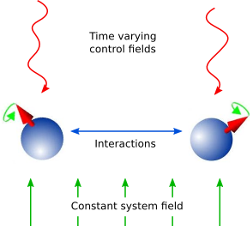
\includegraphics[width=0.5\linewidth]{principles_quantum_control.png}
    \caption{Schematic showing the principle of quantum control\cite{Johansson2013}}
    \label{fig:principles_quantum_control}
\end{figure}

Here we will first consider only finite-dimensional, closed quantum systems. In closed quantum systems the states can be represented by kets, and the transformations on these states are unitary operators. 
The dynamics generators are Hamiltonians. The combined Hamiltonian for the system is given by
$$
H(t)=H_0+\sum_{j=1} u_j(t) H_j
$$
where $H_0$ is the drift Hamiltonian and the $H_j$ are the control Hamiltonians. The $u_j$ are time varying amplitude functions for the specific control.

The dynamics of the system are governed by Schrödingers equation.
$$
\frac{d}{d t}|\psi\rangle=-i H(t)|\psi\rangle
$$

Note we use units where $\hbar=1$ throughout. The solutions to Schrödinger's equation are of the form:
$$
|\psi(t)\rangle=U(t)\left|\psi_0\right\rangle
$$
where $\psi_0$ is the state of the system at $t=0$ and $U(t)$ is a unitary operator on the Hilbert space containing the states. 
$U(t)$ is a solution to the Schrödinger operator equation
$$
\frac{d}{d t} U=-i H(t) U, \quad U(0)=\mathbb{1}
$$

We can use optimal control algorithms to determine a set of $u_j$ that will drive our system from $\left|\psi_0\right\rangle$ to $\left|\psi_1\right\rangle$, this is state-to-state preparation, or drive the system from some arbitary state to a given state $\left|\psi_1\right\rangle$, which is state preparation, or effect some unitary transformation $U_{\text {target }}$, called gate synthesis. 
The latter of these is most important in quantum computation.

%%%%%%%%%%%%%%%%%%%%%%%%%%%%%%%
\section{GRAPE: Gradient Ascent Pulse Engineering}
The GRadient Ascent Pulse Engineering was first proposed in \cite{KHANEJA2005296}. 
Overview of GRAPE algorithm as implemented in QuTip is as follows. 
Solutions to Schrödinger's equation for a time-dependent Hamiltonian are not generally possible to obtain analytically. 
Therefore, a piecewise constant approximation to the pulse amplitudes is made. Time allowed for the system to evolve $T$ is split into $M$ timeslots (typically these are of equal duration), during which the control amplitude is assumed to remain constant. 
\par
In the GRAPE algorithm, the combined Hamiltonian is approximated as a piecewise constant function, where the control amplitudes are assumed to be constant within each timeslot. 
Mathematically, this can be expressed as $H(t) \approx H\left(t_k\right)=H_0+\sum_{j=1}^M u_{j k} H_j$, where $k$ is a timeslot index, $j$ is the control index, and $M$ is the number of controls. 
The variable $t_k$ represents the evolution time at the start of the timeslot, and $u_{jk}$ is the amplitude of control $j$ throughout timeslot $k$. 
The total number of time steps, denoted by $N$, is equal to the total evolution time $T$ divided by the timeslot duration $\delta t$.
Though in my code in chapter \ref{sec:state_preparation}, I set number of time steps and evolution time, which then determines the time slot duration $\delta t$.
\par
Given the piecewise constant approximation of the Hamiltonian, the time evolution operator, also known as the propagator, within each timeslot can be calculated using the matrix exponential: $U_k:=e^{-i H\left(t_k\right) \Delta t_k}$. 
To obtain the overall evolution up to and including any timeslot $k$ (including the full evolution at $k=M$), the propagators for each timeslot are multiplied together in chronological order: $U\left(t_k\right):=U_k U_{k-1} \cdots U_1 U_0$.
\par
To quantify the effectiveness of the control pulses, a figure of merit or fidelity is introduced. 
This metric measures how close the achieved evolution is to the desired target state or transformation, based on the control amplitudes in the timeslots. 
For unitary systems, the typical figure of merit is the normalised overlap between the achieved evolution and the target. 
A more detailed discussion of the figure of merit can be found in chapter \ref{sec:figure_of_merit}.
\par
The optimization problem in GRAPE can be formulated as follows. 
With the piecewise constant approximation, there are now $N\times M$ variables (the control amplitudes in each timeslot) that need to be optimized to minimize the figure of merit. 
This transforms the problem into a finite multi-variable optimization problem, for which many established methods exist. 
These methods are discussed in more detail in chapter \ref{sec:finite_variables_optimization}. In the QuTiP Qtrl GRAPE implementation, the default optimization method is the L-BFGS-B algorithm, which is available through the Scipy library in Python.


%%%%%%%%%%%%%%%%%%%%%%%%%%%%%%%
\section{CRAB: Chopped RAndom Basis}\label{sec:CRAB}
As opposed to GRAPE which optimises time-slice pulse amplitudes, the Chopped RAndom Basis (CRAB) algorithm optimizes the coefficients of a fintie set of functional basis of a chosen functional basis set. 
CRAB algorithm is particularly useful when the pulse complexity is very low \cite{PhysRevLett.106.190501, PhysRevA.84.022326}.
Here we are referring to relatively smooth pulses without singularities or sharp features. 
Such pulses are often more desirable for experiments as actuators at different levels from the pulse generators all the way to the controlled physical often require certain response time. 
In these cases, instead of optimizing the control amplitudes at each time slice, CRAB transforms the optimal control problem into a search over a few parameters by introducing a physically motivated function basis that constructs the pulse. 
This approach significantly reduces the number of optimization parameters compared to the number of time slices needed for accurate quantum dynamics simulations in gradient-based algorithms, often by orders of magnitude. 
As a result, CRAB can efficiently optimize smooth pulses while incorporating realistic experimental constraints.
However, note that CRAB by itself does not guarantee smooth pulses. If a functional basis with basis elements containing discontinuities is chosen, the CRAB solution will inherit those discontinuities.
%%%%%%%%%%%%%%%%%%%%%%%%%%%%%%%
\section{Figure of Merit}\label{sec:figure_of_merit}
For state preparation case, we have the following evolved state fidelity as the figure of merit:
\begin{align*}
    f(\vec{\epsilon}(t)) &= \mathcal{F}(\vec{\epsilon}(t)) \quad \text{state fidelity}\\
    &\equiv \abs{\bra{\psi_{targ}} U(T,\vec{\epsilon}(t)) \ket{\psi_{init}}}^2 \\
    &= \abs{\bra{\psi_{targ}} 
        \mathcal{T}\exp{-\frac{i}{\hbar}\int_0^T dt H(\vec{\epsilon}(t))}
        \ket{\psi_{init}}}^2 \\
    &\text{make the problem numerical, make $\vec{\epsilon}(t)$ a piece-wise constant function with $N=T/\delta t$,} \\
    &\text{$\delta t$ is a parameter, usually set to time resolution of AWG.} \\
    &= \abs{\bra{\psi_{targ}} 
        U_NU_{N-1}...U_1
        \ket{\psi_{init}}}^2, \quad \text{where, } U_k=\exp{\frac{i\delta t}{\hbar}H(\vec{\epsilon}(k\delta t))} \\
\end{align*}
However, for our cavity-DQD composite system the composist system states need to be traced over the qubit state to obtain the cavity state fidelity. 

%%%%%%%%%%%%%%%%%%%%%%%%%%%%%%%
\section{Finite Variables Optimization Algorithms}\label{sec:finite_variables_optimization}
Here we discuss a typical finite-variables optimization scheme.
\begin{equation}
    H(\vec{\epsilon}(t)) = H_0 + \sum_{k=1}^m \epsilon_k(t) H_k
\end{equation}
The goal of quantum optimal control is to find the optimal control field $\vec{\epsilon}(t)$ that optimizes a given function $f(\vec{\epsilon}(t)) = f(H(\vec{\epsilon}(t)))$, where $H(\vec{\epsilon}(t))$ represents the Hamiltonian of the quantum system under the influence of the control field. 
The optimization procedure involves several key steps and considerations.
\par
To effectively optimize a large number of parameters, two important requirements must be met. 
First, an efficient method for calculating the gradients of the cost function with respect to the parameters is essential. 
Second, the optimization landscape should be such that sub-optimal local minima are either sufficiently unlikely or close to the global minimum, ensuring that the optimization algorithm can converge to a satisfactory solution.
\par
Given methods to calculate the cost function and its gradients, two main classes of algorithms can be employed for performing the optimization. 
The first class is line-search methods, which alternate between selecting a direction in the parameter space, radiating from the current point, and performing a one-dimensional minimization along this line to find the minimum. 
The most basic line-search method is gradient descent, which chooses the direction of steepest descent based on the gradient at the current point. 
More advanced methods, such as the Newton method, utilize both the gradient and the Hessian matrix to determine the search direction. 
Quasi-Newton methods, like the L-BFGS algorithm, approximate the Hessian matrix to improve convergence while reducing computational complexity. 
The L-BFGS algorithm is employed in the QuTiP Qtrl GRAPE implementation, and is available through the Scipy library in Python.
The second class of optimization algorithms is trust-region methods, which define a region around the current point within which a quadratic approximation of the cost function is considered reliable, and the optimization is performed within this trust region.
\par
The gradient of the cost function $f(\vec{\epsilon}(t))$ with respect to the control field $\vec{\epsilon}(t)$ plays a crucial role in many optimization algorithms. 
For an analytical function $f(\vec{\epsilon})$, the gradient is given by $\nabla f(\vec{\epsilon}) = \sum_{i=1}^m \frac{\partial f(\vec{\epsilon})}{\partial \epsilon_i} \hat{\epsilon}_i$, where $m$ is the number of control parameters and $\hat{\epsilon}_i$ are unit vectors in the parameter space. 
When dealing with discrete control fields, the gradient can be approximated using the finite difference method. In some cases, calculating or approximating the gradient may be computationally expensive, and alternative optimization algorithms that do not rely on gradient information should be considered.
\par
Once the gradient is calculated, the optimization algorithm takes a step in the direction of the negative gradient, with the step size being a tunable parameter. 
If the step size is too small, the optimization process may be slow, requiring many iterations to converge. 
On the other hand, if the step size is too large, the algorithm may overshoot the minimum and fail to converge to the true optimum. 
The gradient is then recalculated at the new point, and the process is repeated iteratively until a convergence criterion is met, indicating that the optimal control field has been found.

%%%%%%%%%%%%%%%%%%%%%%%%%%%%%%%
\section{Pulse Constraints} \label{sec:pulse_constraints}
When designing optimal control pulses for quantum systems, it is essential to consider the constraints imposed by the experimental setup, particularly those related to the arbitrary waveform generator (AWG). 
The AWG's amplitude and bandwidth limitations can significantly impact the feasibility and performance of the control pulses. 
To incorporate these constraints into the optimization process, one approach is to add a set of constraint terms to the cost function, as shown in the following equation:
\begin{equation*}
    f(\vec{\epsilon}(t)) = \mathcal{F}(\vec{\epsilon}(t)) + \sum_i \lambda_i g_i(\vec{\epsilon})
\end{equation*}
Here, $\mathcal{F}(\vec{\epsilon}(t))$ represents the original cost function, such as the fidelity of the desired quantum operation, while $g_i(\vec{\epsilon})$ are the constraint terms with their respective weights $\lambda_i$.
\par
One of the most common constraints is the pulse amplitude, which is limited by the output power of the AWG. 
To ensure that the control pulses are feasible, we require $\epsilon(t) \le \epsilon_{max}$ for all times $t$. 
There are two main approaches to enforce this constraint: hard cutoff and soft cutoff. 
The hard cutoff approach involves employing an optimization algorithm that naturally allows for such constraints, such as the L-BFGS-B algorithm available in the scipy.optimize module in Python. 
Alternatively, the soft cutoff approach involves parametrizing the optimization problem by introducing a new set of variables $\vec{x}$ and expressing the control amplitudes as $\epsilon_k = \epsilon_{max} \tanh{(x_k)}$. 
This ensures that the control amplitudes always remain within the allowed range.
\par
Another important constraint is the pulse bandwidth, which can be addressed using various methods. 
Soft cutoff methods gradually penalize high-frequency components of the control pulses, while hard cutoff methods impose strict limits on the frequency content. 
Linear frequency-dependent penalties can also be employed, where the penalty term increases linearly with the frequency of the control pulse components.
\par
In addition to the AWG constraints, the finite memory of classical computers poses a challenge when simulating quantum systems with infinite-dimensional Hilbert spaces, such as harmonic oscillators. 
To address this issue, we truncate the Hilbert space by choosing a maximum photon number $n_{ph}$, effectively replacing the infinite-dimensional oscillator with a finite-dimensional qudit.
However, this truncation is only valid if all the relevant system dynamics for the desired state transfers occur within the subspace spanned by ${\ket{0}, \cdots, \ket{n_{ph} - 1}}$.
\par
To ensure that the truncation does not introduce errors in the optimization process, we can modify the optimization problem to find a solution that operates identically under different values of $n_{ph}$. 
By writing the fidelity as a function of the truncation level, $F_{n_{ph}}$, we can formulate the optimization problem as follows:
\begin{equation}
    \stackrel{\text{maximize}}{\vec{\epsilon}} \left( \sum_k F_{n_{ph}+k} (\epsilon(t)) \right) - \left( \sum_i \lambda_i g_i (\epsilon(t)) \right)
\end{equation}
To enforce identical behavior across different truncations, we can add a penalty term that minimizes the discrepancy between the fidelities computed at different truncation levels:
\begin{equation*}
    g_{\text{discrepancy}}(\boldsymbol{\epsilon}(\boldsymbol{t}))=\sum_{k_1 \neq k_2}\left(\mathcal{F}{n{\mathrm{ph}}+k_1}(\boldsymbol{\epsilon}(t))-\mathcal{F}{n{\mathrm{ph}}+k_2}(\boldsymbol{\epsilon}(t))\right)^2
\end{equation*}
This penalty term effectively symmetrizes the cost function with respect to $n_{ph}$.
An alternative and more direct approach is to add a penalty term that minimizes the occupation of the highest photon state ($\ket{n_{ph} - 1}$) in the truncated Hilbert space at any time during the evolution:
\begin{equation*}
    g_{\text{trajectory}}=\sum_{k=1}^N\left|\left\langle n_{\text{ph}}-1 \mid \psi_{\text{fwd}}^{(k)}\right\rangle\right|^2
\end{equation*}
This penalty term encourages the optimization algorithm to find control pulses that keep the system dynamics within the truncated subspace, ensuring the validity of the simulation.
By incorporating these constraints and penalty terms into the optimization problem, we can design control pulses that are not only effective in achieving the desired quantum operation but also feasible to implement experimentally, taking into account the limitations of the AWG and the finite memory of classical computers used for simulations.

%%%%%%%%%%%%%%%%%%%%%%%%%%%%%%%
\section{Troubleshooting Optimization Algorithm}
Here I provide a check list for Troubleshooting the optimization algorithm that I have accumulated during my project. 
However, this list is nonexhaustive and Reinhold provides his version in chapter 4.6, \cite{reinhold2019}.
\begin{enumerate}
    \item Check optimization parameters: 
        \begin{enumerate}
            \item Check that the time given $T = N \delta t$ is appropriate.
                $T$ should be specified in units that are consistent with the units specifying the Hamiltonian. For instance, if the Hamiltonian is specified in GHz, then the time step should be in units of ns.
            \item Check that truncations are sufficiently large. N value appropriate
        \end{enumerate}
    \item check constraints: Completely remove all constraints and penalties, and make sure that the algorithm works in this context before re-introducing them
    \item check termination conditions \\
        Gradient based search algorithms usually have termination conditions specified in terms of the norm of the gradient. 
        It is often necessary to lower the gradient norm threshold for termination to ensure that it does not give up. (gtol in scipy.minimize)
    \item check initial guess: Avoid special initial guesses, this depends on the algorithm. 
        For gradient-based algo, make sure initial gradient is not vanishing.
\end{enumerate}

%%%%%%%%%%%%%%%%%%%%%%%%%%%%%%%
\section{My Codes}
% include: 
% - show what I did to generate the results in next chapter, use what packages and write what codes
This project is entirely conducted in python. The main quantum control libray in python is QuTiP.
This project uses QuTiP library functions for the quantum simulation and GRAPE, CRAB optimization.
Another python library based on QuTip, Krotov is also used in chapter \ref{sec:vac2cat}.
All codes mentioned in chapter \ref{sec:state_preparation} follow a similar structure of defining the Hamiltonian, initial and target states, optimization parameters, then running the optimization algorithm by feeding the above defined variables in into QuTip or Krotov optimization functions and lastly checking optimization result via a forward simulation using both a library function or a self-implemented function. 
A python sample code can be seen in Appendix \ref{sec:sample_code}. Note that the codes in Github are in Jupyter Notebook format, which is more readable and easier for dynamic scientific programming.
Main effort went into determining the appropriate system and optimization parameters values rather than coding these scripts. 
Though with the above said, much effort was put into understanding QuTip source code and at some point correcting or modifying the source code to suit the needs of the project.
For instance, much time was spent in trying to understand how QuTip implements the figure of merit for optimization and modify it to incorporate partial tracing out qubit into the fidelity function. 
However, this did not work out as will be discussed in chapter \ref{sec:further_discussions}.
All the codes mentionded in are available in the GitHub repository \cite{lzl_github_repo}.

%%%%%%%%%%%%%%%%%%%%%%%%%%%%%%%%%%%%%%%%%%%%%%%%%%%%%%%%%%%%%%%
\chapter{State preparation pulse optimization}\label{sec:state_preparation}
Here is a summary of optimization results (shown previously in overview chapter): 

\begin{sidewaystable}
    \begin{tabularx}{\textheight}{|p{4cm}|p{2cm}|X|X|p{2cm}|X|X|X|X|}
    \hline
    name                               & \begin{tabular}[c]{@{}l@{}}physical\\ system\end{tabular}             & \begin{tabular}[c]{@{}l@{}}initial\\ state\end{tabular} & \begin{tabular}[c]{@{}l@{}}target\\ state\end{tabular}  & \begin{tabular}[c]{@{}l@{}}ops\\ algo\end{tabular} & N(Fock space truncation)     & \begin{tabular}[c]{@{}l@{}} time \\ discre- \\ -tisation\end{tabular} & \begin{tabular}[c]{@{}l@{}}pulse\\ length \\ (ns) \end{tabular} & \begin{tabular}[c]{@{}l@{}}final\\ fidelity\\ (simulation)\end{tabular} \\ \hline
    single\_qubit                      & \begin{tabular}[c]{@{}l@{}}single\\ qubit\end{tabular}                & \begin{tabular}[c]{@{}l@{}}ground\\ state\end{tabular}  & \begin{tabular}[c]{@{}l@{}}excited\\ state\end{tabular} & GRAPE                                              & NIL & 1000                                                           & 18                                                     & 0.9999                                                      \\ \hline
    vaccuum2coherent                       & \begin{tabular}[c]{@{}l@{}}cavity\\ coupled to\\ a qubit\end{tabular} & $\psi_{i1}$                                             & $\psi_{f1}$                                             & GRAPE                                              & 5     & 100                                                            & 1                                                      & 0.9999                                                        \\ \hline
    unselective\_spin\_flip            & \begin{tabular}[c]{@{}l@{}}cavity\\ coupled to\\ a qubit\end{tabular} & $\psi_{i2}$                                                        & $\psi_{f2}$                                                       & GRAPE                                              & 16    & 500                                                            & 1                                                      & 0.9995                                                      \\ \hline
    selective\_spin\_flip              & \begin{tabular}[c]{@{}l@{}}cavity\\ coupled to\\ a qubit\end{tabular} & $\psi_{i3}$                                                        & $\psi_{f3}$                                                       & GRAPE                                              & 16    & 100000                                                         & 500                                                    & 0.9994                                                      \\ \hline
    \begin{tabular}[c]{@{}l@{}}selective\_spin\_flip\\ \_constraints\end{tabular} & \begin{tabular}[c]{@{}l@{}}cavity\\ coupled to\\ a qubit\end{tabular} & $\psi_{i3}$             & $\psi_{f3}$                                                        & GRAPE                                              & 16    & 100000                                                         & 500                                                    & 0.9992                                                      \\ \hline
    vacuum2cat                            & \begin{tabular}[c]{@{}l@{}}cavity\\ coupled to\\ a qubit\end{tabular} & $\psi_{i4}$                                                        & $\psi_{f4}$                                                        & GRAPE                                              & 16    & 100000                                                         & 5000                                                   & 0.9529                                                                        \\ \hline
    vacuum2cat                            & \begin{tabular}[c]{@{}l@{}}cavity\\ coupled to\\ a qubit\end{tabular} & $\psi_{i4}$                                                        & $\psi_{f4}$                                                        & KROTOV                                              & 16    & 100000                                                         & 5000                                                   & 0.9995                                                                       \\ \hline
    \end{tabularx}
\end{sidewaystable}

where, initial and target states are given by: 
\begin{align*}
    % vac2coherent
    \text{vac2coherent} \\
    \psi_{i1} &= \ket{0}_{\text{cavity}} \otimes \ket{0}_{\text{qubit}} \\
    \psi_{f1} &= \ket{\alpha}_{\text{cavity}} \otimes \ket{0}_{\text{qubit}} \\
    % unselective
    \text{unselective} \\
    \psi_{i2} &= \frac{1}{\sqrt{2}} (\ket{0}_{\text{cavity}} \otimes \ket{0}_{\text{qubit}} 
                + \ket{1}_{\text{cavity}} \otimes \ket{0}_{\text{qubit}})\\
    \psi_{f2} &= \frac{1}{\sqrt{2}} (\ket{0}_{\text{cavity}} \otimes \ket{1}_{\text{qubit}} 
                + \ket{1}_{\text{cavity}} \otimes \ket{1}_{\text{qubit}})\\
    % selective
    \text{selective} \\
    \psi_{i3} &= \frac{1}{\sqrt{2}} (\ket{0}_{\text{cavity}} \otimes \ket{0}_{\text{qubit}} 
                + \ket{1}_{\text{cavity}} \otimes \ket{0}_{\text{qubit}})\\
    \psi_{f3} &= \frac{1}{\sqrt{2}} (\ket{0}_{\text{cavity}} \otimes \ket{0}_{\text{qubit}} 
                + \ket{1}_{\text{cavity}} \otimes \ket{1}_{\text{qubit}})\\
    % vac2cat
    \text{vac2cat} \\
    \psi_{i1} &= \ket{0}_{\text{cavity}} \otimes \ket{0}_{\text{qubit}} \\
    \psi_{f1} &= \ket{\alpha}_{\text{cavity}} \otimes \ket{0}_{\text{qubit}} 
                + \ket{-\alpha}_{\text{cavity}} \otimes \ket{0}_{\text{qubit}} \\
\end{align*}


%%%%%%%%%%%%%%%%%%%%%%%%%%%%%%%
\section{Starting With a Simple Diagnostic Pulse, Single Qubit System}
To verify that I have a working code that can optimize a pulse, 
I will start with a simple qubit flip operation of a single-qubit system.
The purpose of this chapter is to show that the algorigm is indeed running optimization
by recovering analytically solvable state-to-state transer using pulse optimization. 
\par
In the following example, we consider using the CRAB algorithm as implemented in the 
qutip python library. In qutip, the ctrlpulseoptim.optimize\_pulse\_unitary function is used 
to optimize pulse shapes to minimize the fidelity error, which is equivalent maximising the fidelity to an optimal value of 1.
\par
The Hamiltonian of a single qubit system with arbitrary control is give by, 
\begin{equation}
    H(t) = \frac{\hbar \omega_0}{2} \sigma_z + \epsilon_x(t)\sigma_x + \epsilon_y(t)\sigma_y 
\end{equation}
where, $\epsilon_x(t), \epsilon_y(t)$ are control pulses.  
\par
Consider a special case of the above general case. 
\begin{equation}
    H_1(t) = \frac{\hbar \omega_0}{2} \sigma_z + \frac{\hbar \omega_1}{2}(\sigma_x\cos{\omega t} + \sigma_y\sin{\omega t})    
\end{equation}

% TODO: add derivation here
From Valerio's note, via frame rotation, starting from $\ket{\psi_{init}} = \ket{+\hat{z}}$, 
we have evoloved state, 
\begin{equation}
    |\psi(t)\rangle=e^{-i \omega t / 2}[\cos (\Omega t / 2)-i \cos \theta \sin (\Omega t / 2)]|+\hat{z}\rangle-i e^{i \omega t / 2} \sin \theta \sin (\Omega t / 2)|-\hat{z}\rangle
\end{equation}
where, 
$$
\Omega=\sqrt{\left(\omega_0-\omega\right)^2+\omega_1^2} \\
\cos \theta=\frac{\omega_0-\omega}{\Omega}
$$

Suppose we want to achieve a state-to-state preparation from $\ket{+\hat{z}}$ to $\ket{-\hat{z}}$,  
$$
P_{+\hat{z} \rightarrow-\hat{z}}(t) = \sin ^2 \theta \sin ^2(\Omega t / 2)=\left(\frac{\omega_1}{\Omega}\right)^2 \sin ^2(\Omega t / 2)
$$
With $H_1(t)$, $P_{+\hat{z} \rightarrow-\hat{z}}(t)$ only goes to 1 if 
\begin{enumerate}
    \item $\omega_1 = \Omega$, i.e. $\omega = \omega_0$.
    \item $\omega_1 = \frac{\pi}{T}$ (with evolution time T fixed, smallest frequency needed)
\end{enumerate}
Now we run the pulse optimization and compare with analytical result.
\\
Let t = evo\_time = T
\\
Defining the time evolution parameters:
- To solve the evolution the control amplitudes are considered constant within piecewise timeslots, hence the evolution during the timeslot can be calculated using U(t\_k) = expm(-iH(t\_k)dt). 
- Combining these for all the timeslots gives the approximation to the evolution from an initial state $\psi_0$ at t=0 to $U(T)\psi_0$ at the t=evo\_time. The number of timeslots and evo\_time have to be chosen such that the timeslot durations (dt) are small compared with the dynamics of the system.
- set drift frequency $\omega_0$ to some number, at resonance $\omega = \omega_0$, for state to state preparation to happen at the end of pulse, require $\omega_1 = \frac{\pi}{T}$.
\par
Next, we set the initial guess pulses where the pulse optimization algorithm starts. 
During the each iteration of the optimization, the Nelder-Mead algorithm calculates a new set of coefficients that improves the currently worst set among all set of coefficients. For details see [1,2] and a textbook about static search methods. 
The algorithm continues until one of the termination conditions defined above has been reached. If undesired results are achieved, rerun the algorithm and/or try to change the number of coefficients to be optimized for, as this is a very crucial parameter.  

% TODO: add here the results from GRAPE and CRAB, and discuss their issues with the intended goal\
The optimization parameters are: 
\begin{enumerate}
    \item Number of time slots, n\_ts = 1000
    \item Time allowed for the evolution, evo\_time = 18
    \item Fidelity error target, fid\_err\_targ = 1e-6
    \item Maximum iterations for the optimization algorithm, max\_iter = 10000
    \item Maximum (elapsed) time allowed in seconds, max\_wall\_time = 120
    \item initial pulse, p\_type = 'SINE'
\end{enumerate}

The optimized pulses are: 
\begin{figure}[H]
    \centering
    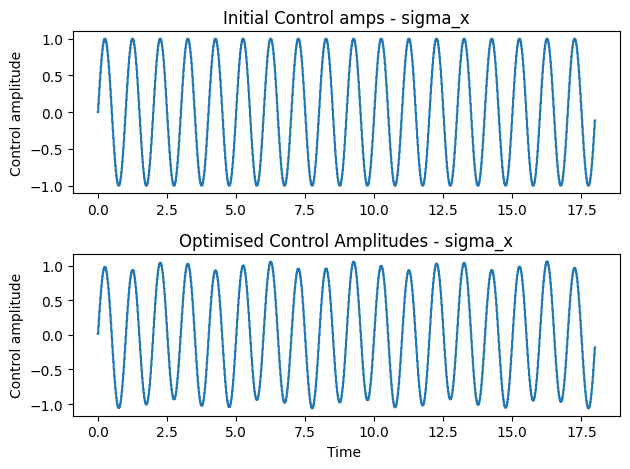
\includegraphics[width=0.95\linewidth]{single_qubit_control1.png}
    \caption{single qubit control 1 pulse}
    \label{fig:single_qubit_control1}
\end{figure}
\begin{figure}[H]
    \centering
    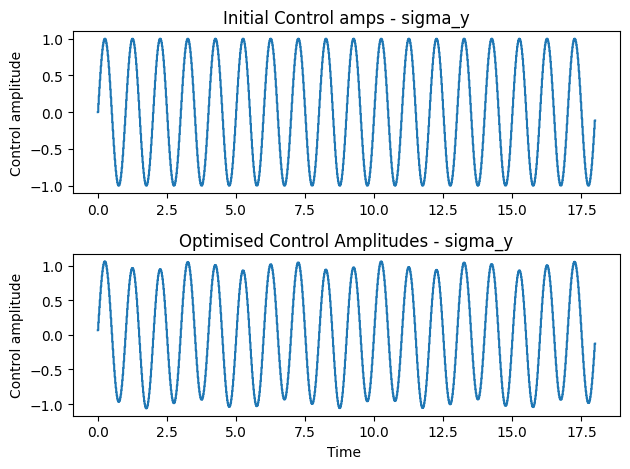
\includegraphics[width=0.95\linewidth]{single_qubit_control2.png}
    \caption{single qubit control 2 pulse}
    \label{fig:single_qubit_control2}
\end{figure}

We can see that the optimized pulses are only slightly modified from the initial guess pulses. 
This is because firstly to drive a single qubit flip is but a simple rabi drive and the initial SINE pulse frequency has been chosen to match the qubit frequency. 
Secondly, the GRAPE algorithm optimizes by modifying time-slice pulse amplitudes, thus leading to small overall waveform change for a simple optimization task.
\par
Though the exact analytical solution couldn't be recovered from numetical optimization as numerical optimization searches through a huge optimization landscape where the analytical solution is only a special case, 
the algorithm can be crudely verified to be running by a forward simulation which shows the optimized evolved state fidelity to be 0.9999367235643194. 

% TODO: describe the simple self-implemented forward simulation code here and add graphs

% TODO: add the code in annex and add link to github

% TODO: discuss why is there a qutip simulation and a self-implemented simulation

%%%%%%%%%%%%%%%%%%%%%%%%%%%%%%%
\section{Diagnostic Pulse: Cavity Vacuum to Cavity Coherent State}
Having tested the code on a single qubit system, we now move on to a more complex system that I am eventually interested in. 
In this code, we consider a cavity coupled to a single qubit.
%TODO:
% - revise Reinhold thesis
% - vet the following chapter with chiyuan, 几个哈密度量的物理意义 + 他们之间的转换  
% - discuss that we are just looking at area under curve here, code to calcualte area under curve
For this physical system, we have drift Hamiltonian, 
from Reinhold PhD thesis (2.13) \cite{reinhold2019}: 
\begin{equation}
    H_d = \omega_q a^\dagger a + \frac{\omega_z}{2} \sigma_z + \frac{\chi}{2} a^\dagger a \sigma_z
\end{equation}
It can be shown that it's equivalent to: %TODO: vet this
\begin{equation}
    \begin{aligned}
    H_d &= g\left( \hat{\sigma}_+ \hat{\sigma}_- + \hat{a}^{\dagger}\hat{a}\hat{\sigma}_z \right) \\
    &= g \left( \frac{1}{2}(1+\hat{\sigma}_x) + \hat{n}\hat{\sigma}_z\right)
\end{aligned}
\end{equation}

where, $g$ is the cavity-qubit coupling strength which is set to be $50*2 \pi MHz$ here, as given by experiment
% TODO: ask chiyuan about g value, cite paper for this valu 
\par
For this physical system we have both cavity and auxiliary qubit contorl, in the form of control Hamiltonian: 
\begin{equation}
    H_c = \epsilon_c(t) \hat{a} + \epsilon_T(t) \hat{\sigma}_- + h.c.
\end{equation}

where, 
\begin{itemize}
    \item $\epsilon_c(t)$ is the contorl signal to cavity
    \item $\epsilon_T(t)$ is the control signal to ancilliary qubit
\end{itemize} 

with $\hat{\sigma}_- = \frac{1}{2} \hat{\sigma}_x - \frac{i}{2}\hat{\sigma}_y$, 
rewrite $H_c$ as following for ease of implementation using QuTip:
\begin{equation}
    H_c = \epsilon_c(t) \hat{a} + \epsilon_T(t) (\frac{1}{2} \hat{\sigma}_x - \frac{i}{2}\hat{\sigma}_y) + h.c.
\end{equation}
Assuming that the control signals $\epsilon_c(t), \epsilon_T(t)$ are real, and ignoring scalar constants, we have 
$$
H_c = \epsilon_c(t) (\hat{a}+\hat{a}^{\dagger}) + \epsilon_T(t) \hat{\sigma}_x
$$

Initial and target states: 
\begin{equation}
    \begin{aligned}
    \ket{\psi_{\text{initial}}} &= \ket{\alpha} \\
    \ket{\psi_{\text{final}}} &= \ket{\alpha} + \ket{-\alpha}
\end{aligned}
\end{equation}


For testing the code, consider
\begin{equation}
    \begin{aligned}
        \ket{\psi_{\text{initial}}} &= \ket{0} \\
        \ket{\psi_{\text{final}}} &= \ket{\alpha}
    \end{aligned}
\end{equation}


The optimization algorithm settings used in this example are: 
\begin{itemize}
    \item Number of time slots, n\_ts = 100
    \item Time allowed for the evolution, evo\_time = 1
    \item Fidelity error target, fid\_err\_targ = 1e-4
    \item Maximum iterations for the optisation algorithm, max\_iter = 100000
    \item Maximum (elapsed) time allowed in seconds, max\_wall\_time = 10000
    \item optimization algorithm: GRAPE
\end{itemize}

The initial and optimised pulses:

\begin{figure}[H]
    \centering
    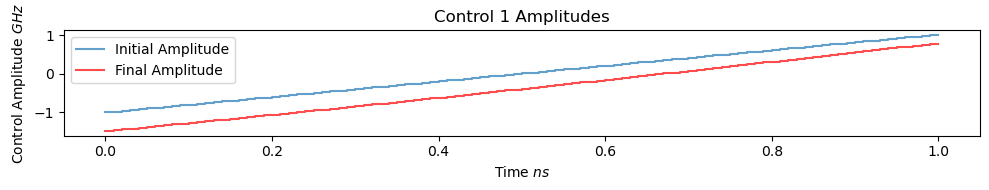
\includegraphics[width=0.95\linewidth]{vac2coherent_control1.png}
    \caption{vacuum to coherent control 1 pulse}
    \label{fig:vac2coherent_control1}
\end{figure}
\begin{figure}[H]
    \centering
    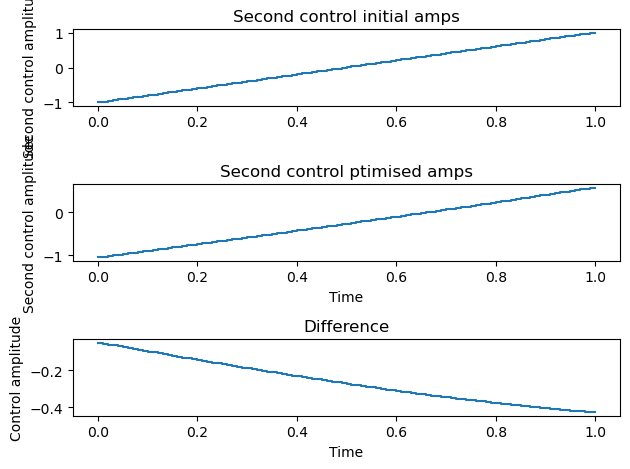
\includegraphics[width=0.95\linewidth]{vac2coherent_control2.png}
    \caption{vacuum to coherent control 2 pulse}
    \label{fig:vac2coherent_control2}
\end{figure}

Forward simulation is as follows: 
\begin{figure}[H]
    \centering
    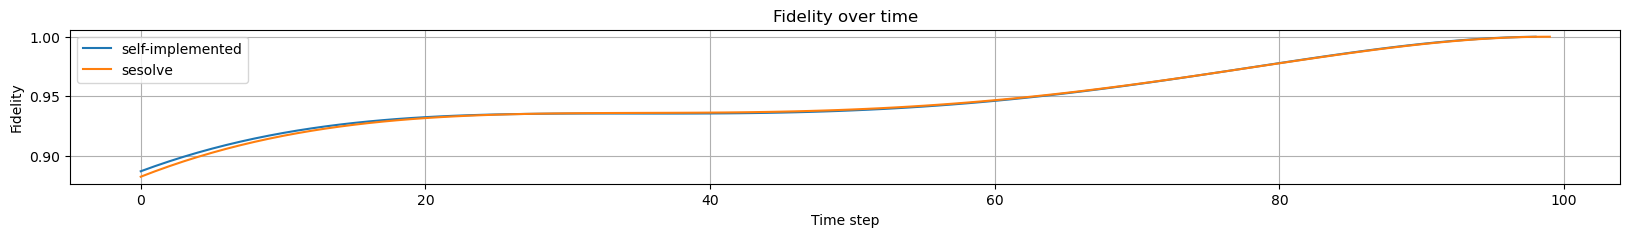
\includegraphics[width=0.95\linewidth]{vac2coherent_simulate.png}
    \caption{vacuum to coherent forward simulate}
    \label{fig:vac2coherent_simulate}
\end{figure}

To verify whether the cavity state basis truncation $N$ is large enough, i.e. 
whether the optimziation result has converged with respect to $N$, consider: 
\begin{enumerate}
    \item Run the optimization with the same algorithm settings and same initial guess, but with different $N$ values. 
        Then plots the optimized pulses ran with different $N$ values on the same plot. 
    \item Simulate the evolution of the system with the optimized pulses, but with a range of higher $N$ values. 
\end{enumerate}

\begin{figure}[H]
    \centering
    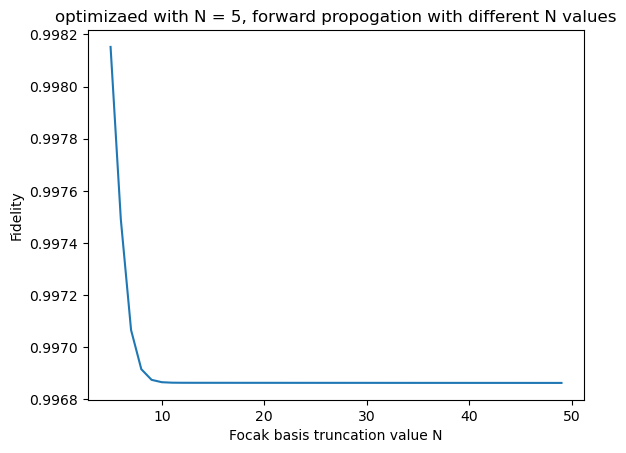
\includegraphics[width=0.95\linewidth]{vac2coherent_N_convergence.png}
    \caption{cavity state Fock basis truncation $N$ convergence}
    \label{fig:vac2coherent_N_convergence}
\end{figure}

\begin{figure}[H]
    \centering
    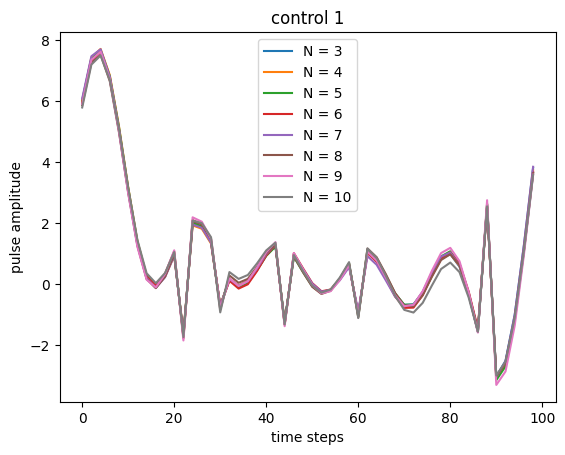
\includegraphics[width=0.95\linewidth]{check_convergence_control1.png}
    \caption{cavity state Fock basis truncation $N$ convergence}
    \label{fig:check_convergence_control1}
\end{figure}

\begin{figure}[H]
    \centering
    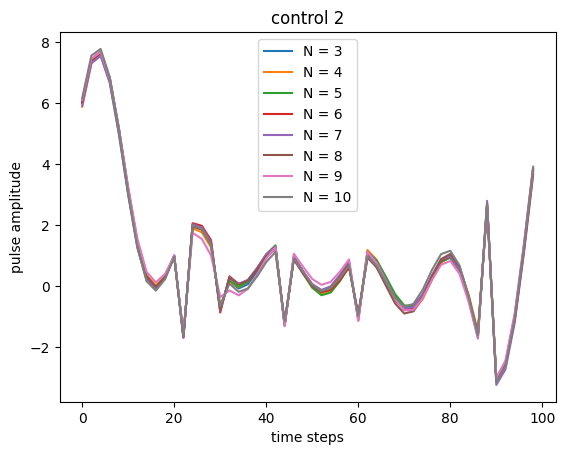
\includegraphics[width=0.95\linewidth]{check_convergence_control2.png}
    \caption{cavity state Fock basis truncation $N$ convergence}
    \label{fig:check_convergence_control2}
\end{figure}

%%%%%%%%%%%%%%%%%%%%%%%%%%%%%%%
\section{Diagnostic Pulse: Unselective Spin Flip, Cavity Coupled With Single Qubit(effective)}
Going from a cavity cavuum state to a cavity coherent state analytically requires only a displacement operation
which requires only a control pulse to the cavity. Hence, in the previous disagnostic scenario the full Hamiltonia
with all three (real) control channels were not used.
\par
Here we consider the full system Hamiltonian (cavity + auxiliary qubit + coupling terms)
drift Hamiltoinan is given by, 
\begin{equation}
    H_d = \text{wr} * n_{\text{cavity}} + \text{Ez} * \sigma_z + \text{chi} * \sigma_z * (n_{\text{cavity}} + 1/2 )    
\end{equation}
where parameters of the physical system are:
\par
(notet that energy terms have unit $GHz$ and time terms have unit $ns$)
% TODO: ask chiyuan how to get these numbers
\begin{itemize}
    \item cavity frequency, wr = $2 \pi$
    \item qubit anharmonicity Ez = $0.44 \pi$
    \item qubit-cavity coupling strength chi = $0.007$
\end{itemize}

Real control channels in the Hamiltonain are given by (each term comprises a channel): 
\begin{equation}
    H_c = a + a^{\dagger} + -1j*(a - a^{\dagger}) + \sigma_x    
\end{equation}

The initial and target states for this pulse optimization code are: 
\begin{align*}
    \psi_0 &= \frac{1}{\sqrt{2}} (\ket{0}_{\text{cavity}} \otimes \ket{0}_{\text{qubit}} 
                + \ket{1}_{\text{cavity}} \otimes \ket{0}_{\text{qubit}})\\
    \psi_{\text{targ}} &= \frac{1}{\sqrt{2}} (\ket{0}_{\text{cavity}} \otimes \ket{1}_{\text{qubit}} 
                + \ket{1}_{\text{cavity}} \otimes \ket{1}_{\text{qubit}})\\
\end{align*}

where the qubit state is flipped irrepsective of the cavity state
\par
The final optimization algorithm parameters are:
%TODO: ask chiyuan how the appropriate pulse length is calcualted
\begin{itemize}
    \item optimization algorithm: GRAPE
    \item Number of time slots, n\_ts = 500
    \item Time allowed for the evolution, evo\_time = 1
    \item Fidelity error target, fid\_err\_targ = 1e-3
    \item Maximum iterations for the optisation algorithm, max\_iter = 1000
    \item Maximum (elapsed) time allowed in seconds, max\_wall\_time = 120
    \item initial guess pulse type, p\_type = 'LIN'
\end{itemize}

The inital and optimized pulses are: 
\begin{figure}[H]
    \centering
    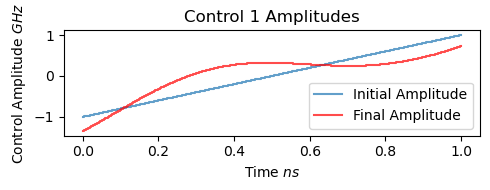
\includegraphics[width=0.95\linewidth]{unselective_spin_flip_control1.png}
    \caption{unselective spin flip control 1 pulse amplitudes}
    \label{fig:unselective_spin_flip_control1}
\end{figure}
\begin{figure}[H]
    \centering
    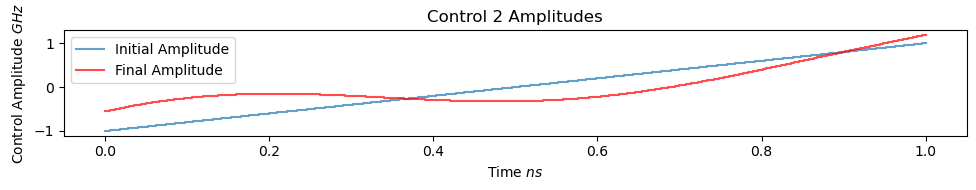
\includegraphics[width=0.95\linewidth]{unselective_spin_flip_control2.png}
    \caption{unselective spin flip control 2 pulse amplitudes}
    \label{fig:unselective_spin_flip_control2}
\end{figure}
\begin{figure}[H]
    \centering
    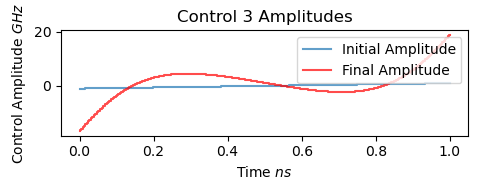
\includegraphics[width=0.95\linewidth]{unselective_spin_flip_control3.png}
    \caption{unselective spin flip control 3 pulse amplitudes}
    \label{fig:unselective_spin_flip_control3}
\end{figure}

Forward simulation is given below to ensure that pulse optimization has run properly. 
\par
Simulation gives: 
\begin{itemize}
    \item sesolve final fidelity:  0.9995869703894827
    \item self-implemented final fidelity:  0.9995575205270999
\end{itemize}
\begin{figure}[H]
    \centering
    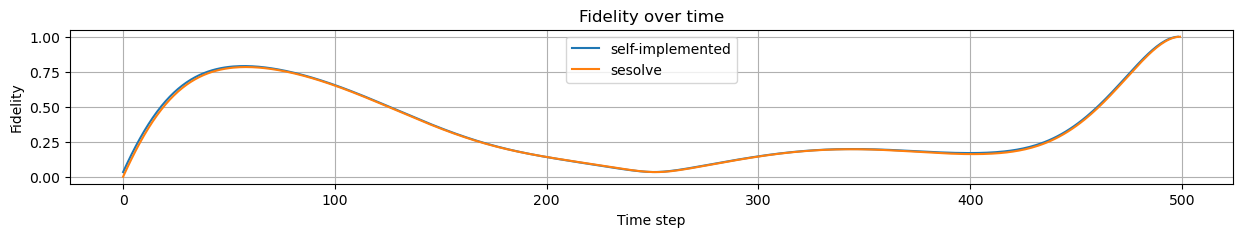
\includegraphics[width=0.95\linewidth]{unselective_spin_flip_simulation.png}
    \caption{unselective spin flip forward simulation}
    \label{fig:unselective_spin_flip_forward_simulation}
\end{figure}

%%%%%%%%%%%%%%%%%%%%%%%%%%%%%%%
\section{Diagnostic Pulse: Selective Spin Flip, Cavity Coupled With Single Qubit (effective)}

For this scenario, the drift and contorl Hamiltonian terms are same as in the previous chapter. We are interested in this state 
preparation because as achieved by Krastanov et al.(2015) \cite{Krastanov2015} which gave a contruction for how to achieve arbitrary 
operation on dispersively coupled cQED systems using a set of two opeartions: displacements and selective number-dependent arbitrary phase (SNAP) operations. 
SNAP operations allow an arbitrary set of relative phases to be applied to different photon number states, and can be represented with the form
\begin{equation}
    S(\vec{\theta}) = \sum_k e^{i\theta_k} \ket{k}\bra{k}
\end{equation}

Clearly, SNAP operations require selective spin rotations of which selective spin flip is a special case.
\par
State preparation optimization target is as follow: 
\begin{align*}
    \psi_0 &= \frac{1}{\sqrt{2}} (\ket{0}_{\text{cavity}} \otimes \ket{0}_{\text{qubit}} 
                + \ket{1}_{\text{cavity}} \otimes \ket{0}_{\text{qubit}})\\
    \psi_{\text{targ}} &= \frac{1}{\sqrt{2}} (\ket{0}_{\text{cavity}} \otimes \ket{0}_{\text{qubit}} 
                + \ket{1}_{\text{cavity}} \otimes \ket{1}_{\text{qubit}})\\
\end{align*}
(where qubit spin flip is selective on cavity state)
% TODO: 问chiyuan,selective spin flip 和 unselective spin flip 的主要区别在哪
% discuss 
% - selective spin flip 和 unselective spin flip 的主要区别在哪
% - why is selective spin flip the next step
% - discuss pulse amplitude constraint
% - ask chiyuan how the appropriate pulse length is calcualted
% - figure out about the cavity state going to higher photon number state inbetween state transition
\par
The best optimization result that was obtained by tuning the optimization script from 
previous chapter is as follow. 
\\
The final optimization algorithm parameters are:
\begin{itemize}
    \item optimization algorithm: GRAPE
    \item Number of time slots, n\_ts = 100000
    \item Time allowed for the evolution, evo\_time = 500
    \item Fidelity error target, fid\_err\_targ = 1e-8
    \item Maximum iterations for the optisation algorithm, max\_iter = 10000
    \item Maximum (elapsed) time allowed in seconds, max\_wall\_time = 7200
    \item initial guess pulse type, p\_type = 'SINE'
\end{itemize}

The inital and optimized pulses are: 
\begin{figure}[H]
    \centering
    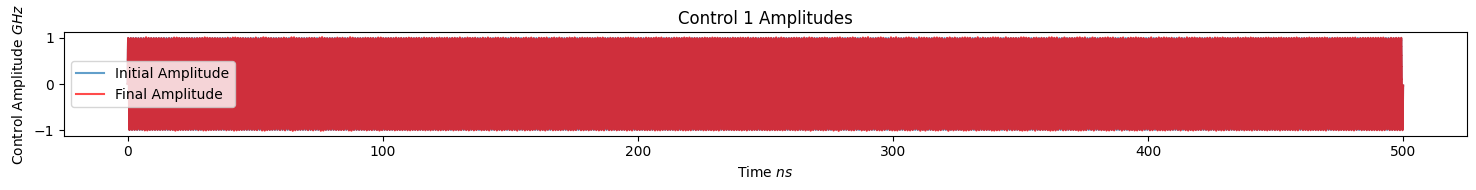
\includegraphics[width=0.95\linewidth]{selective_spin_flip_GRAPE_control1.png}
    \caption{selective spin flip control 1 pulse amplitudes}
    \label{fig:selective_spin_flip_control1}
\end{figure}
\begin{figure}[H]
    \centering
    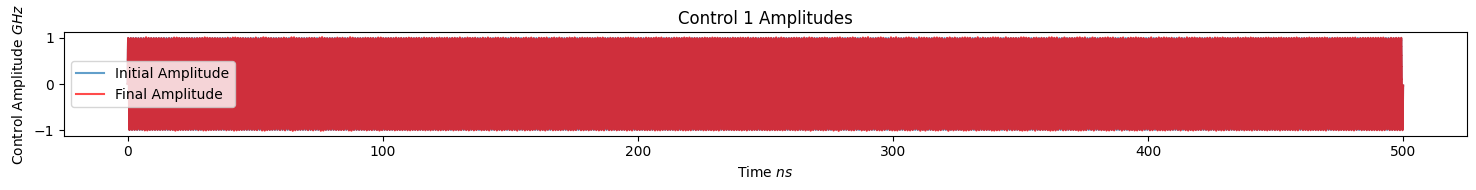
\includegraphics[width=0.95\linewidth]{selective_spin_flip_GRAPE_control1.png}
    \caption{selective spin flip control 2 pulse amplitudes}
    \label{fig:selective_spin_flip_control2}
\end{figure}
\begin{figure}[H]
    \centering
    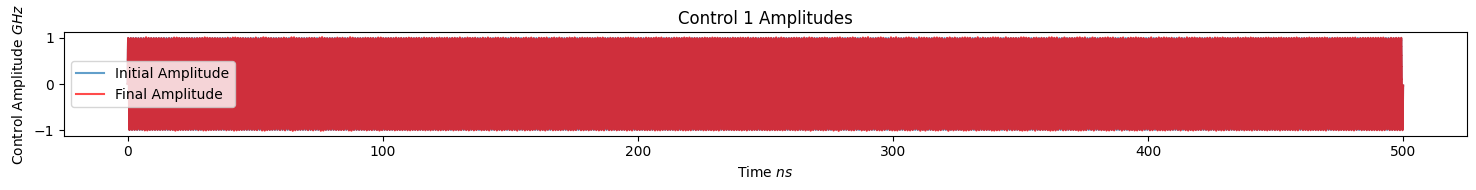
\includegraphics[width=0.95\linewidth]{selective_spin_flip_GRAPE_control1.png}
    \caption{selective spin flip control 3 pulse amplitudes}
    \label{fig:selective_spin_flip_control3}
\end{figure}
\begin{figure}[H]
    \centering
    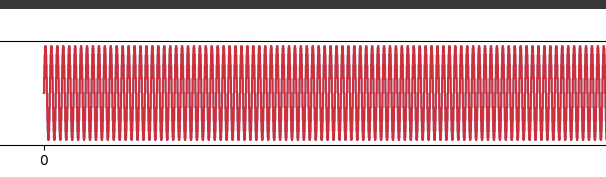
\includegraphics[width=0.95\linewidth]{selective_spin_flip_GRAPE_control1_zoomin.jpeg}
    \caption{selective spin flip control 1 pulse amplitudes zoom in}
    \label{fig:selective_spin_flip_GRAPE_control1_zoomin}
\end{figure}

The control pulses have very fast oscillations due to the large number of time slices.
Zooming into control 1 pulse amplitudes, as shown in fig \ref{fig:selective_spin_flip_GRAPE_control1_zoomin},
we see that the pulse is fairly smooth. However, this fast oscillation is still not desirable and preferably gotten rid of. 
Another reason that might have contributed to this fast oscillation is the background frequency of the cavity and qubit 
of which the control pulses are trying to cancel out. One way to partially deal with this fast oscillation issue is to work
with the Hamiltonian in the rotating frame which will be tried out in the next chapter when cavity vacuum state to cavity cat state
is being optimized.  

Forward simulation is given below to ensure that pulse optimization has run properly. 
\par
Simulation gives: 
\begin{itemize}
    \item sesolve final fidelity:  0.9994876128337873
    \item cavity ptrace fidelity:  0.9997184822307845
    \item qubit ptrace fidelity:  0.999999719275808
    \item self-implemented final fidelity:  0.9997005493228243
\end{itemize}
\begin{figure}[H]
    \centering
    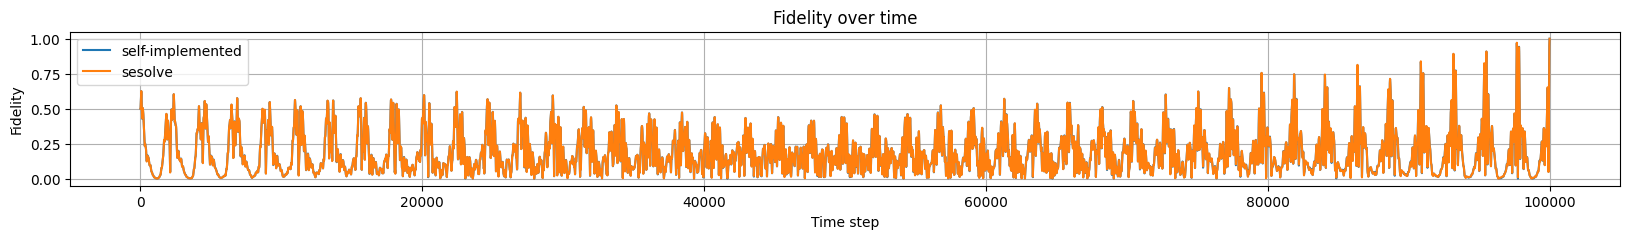
\includegraphics[width=0.95\linewidth]{selective_spin_flip_GRAPE_simulation.png}
    \caption{selective spin flip forward simulation}
    \label{fig:selective_spin_flip_forward_simulation}
\end{figure}


A particular analytical solution as given by Chiyuan already gives fidelity of $~0.98$.
            We expect a higher fidelity from a numerical optimization solution. 
            % TODO: ask chiyuan for analytical solution and put here
\par
However, this numerical solution has the folowing issues.
The optimzied pulses go beyong the amplitude constrains that required for the effective Hamiltonian to be valid. 
When the pulse amplitdes constrained are supplied to the optimziation algorithms, the results are not very satisfactory. 
% TODO: try the code with pulse amplitude constraints}
\par
The following run has two modifications: 
\begin{itemize}
    \item initial guess pulse is changed from sindusoidal to linear to see whether this improves the fast oscillation issue
    \item Pulse amplitude constraints are added to the optimization algorithm
\end{itemize}
However, as can be seen from the optimized pulses below, the fast oscillation issue is not resolved well. 
This is especially so for control 3.
\par
The inital and optimized pulses are: 
\begin{figure}[H]
    \centering
    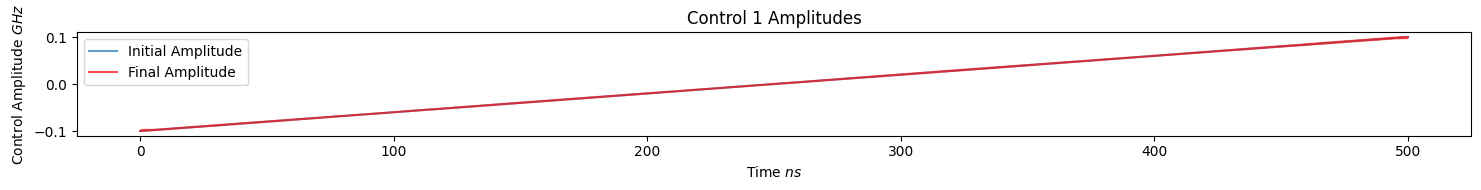
\includegraphics[width=0.95\linewidth]{selective_spin_flip_GRAPE_500,_100_000_LIN_constraints_control1.png}
    \caption{selective spin flip control 1 pulse amplitudes}
    \label{fig:selective_spin_flip_constrains_control1}
\end{figure}
\begin{figure}[H]
    \centering
    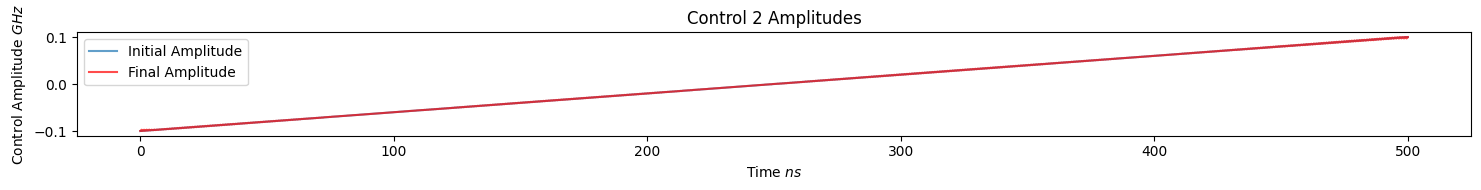
\includegraphics[width=0.95\linewidth]{selective_spin_flip_GRAPE_500,_100_000_LIN_constraints_control2.png}
    \caption{selective spin flip control 2 pulse amplitudes}
    \label{fig:selective_spin_flip_constrains_control2}
\end{figure}
\begin{figure}[H]
    \centering
    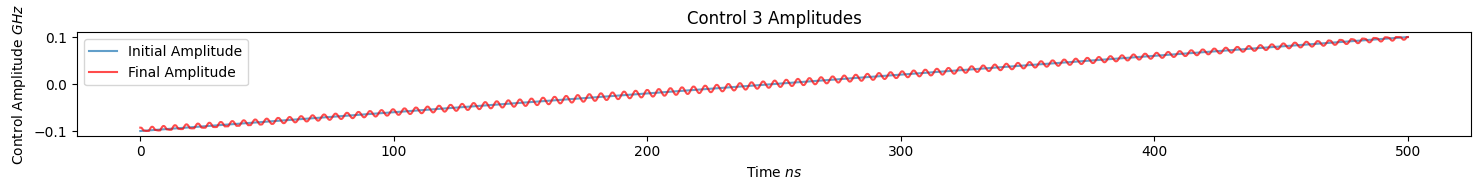
\includegraphics[width=0.95\linewidth]{selective_spin_flip_GRAPE_500,_100_000_LIN_constraints_control3.png}
    \caption{selective spin flip control 3 pulse amplitudes}
    \label{fig:selective_spin_flip_constrains_control3}
\end{figure}

Forward simulation is given below to ensure that pulse optimization has run properly. 
\\
Simulation gives: 
\begin{itemize}
    \item sesolve final fidelity:  0.9992259750482354
    \item cavity ptrace fidelity:  0.9992525011412332
    \item qubit ptrace fidelity:  0.9992706948956261
    \item self-implemented final fidelity:  0.9999937323329505
\end{itemize}
\begin{figure}[H]
    \centering
    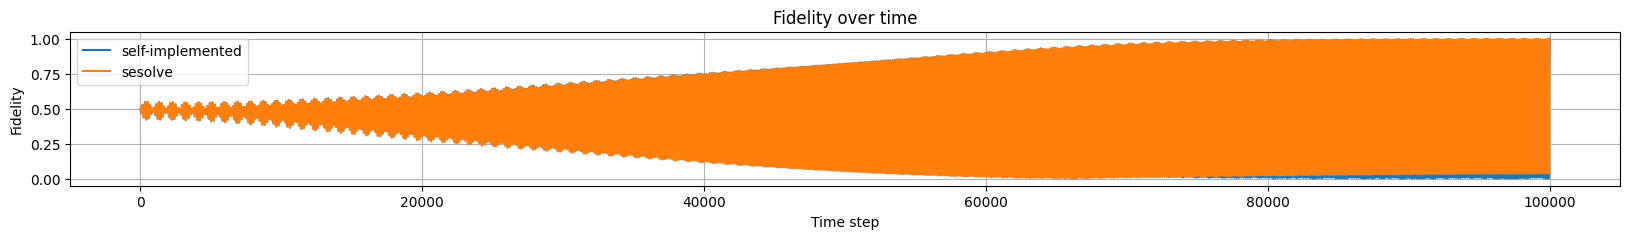
\includegraphics[width=0.95\linewidth]{selective_spin_flip_GRAPE_500,_100_000_LIN_constraints_simulation.png}
    \caption{selective spin flip forward simulation}
    \label{fig:selective_spin_flip_constraints_forward_simulation}
\end{figure}

At this point, we continued varying the parameters (puse length, number of slices, initial guess pulse, etc.). 
However, none gave optimization results where fidelity, pulse amplitude, pulse smoothness and fast oscillation issue 
are all accounted for satisfactorily. 

%%%%%%%%%%%%%%%%%%%%%%%%%%%%%%%
\section{Vacuum to Cat State, Cavity Coupled With Single Qubit (effective)}\label{sec:vac2cat}
In this chapter, we finally get to do a state preparation optimization of cavity vacuum state to cavity cat state.
The drift and control Hamiltonian terms are same as in the previous chapter.

The initial and target states for this pulse optimization code are:
\begin{align}
    \psi_{\text{initial}} &= \ket{0}_{\text{cavity}} \otimes \ket{0}_{\text{qubit}} \\
    \psi_{\text{target}} &= \ket{\alpha}_{\text{cavity}} \otimes \ket{0}_{\text{qubit}} 
                + \ket{-\alpha}_{\text{cavity}} \otimes \ket{0}_{\text{qubit}} \\
\end{align}

The most efficient way to do this is to optimize for the cavity state alone by tracing out the qubit state when calculating state fidelity. 
However, the QuTip package does not support this feature. I attemped to modify QuTip source code to allow for this feature but failed. 
One might naively think that QuTip calculates state fidelity at the end of each optimization iteration. 
Intead, QuTip calculates the state fidelity throughout the entire control pulse evolution for some caching purposes that improves the overall performance of the optimization algorithm. 
Here, a problem arises as tracing out qubit state in the middle of a pulse is not valid. 
% WHY? 
\par
Hence, composite state of the cavity and qubit was still used for optimization which restricts the search space to smaller than ideal. 
However, the optimization results as shown below were not very satisfacotry. 
\\
The final optimization algorithm parameters are:
%TODO: ask chiyuan how the appropriate pulse length is calcualted
\begin{itemize}
    \item optimization algorithm: GRAPE
    \item Number of time slots, n\_ts = 100000
    \item Time allowed for the evolution, evo\_time = 5000
    \item Fidelity error target, fid\_err\_targ = 1e-8
    \item Maximum iterations for the optimization algorithm, max\_iter = 10000
    \item Maximum (elapsed) time allowed in seconds, max\_wall\_time = 21600
    \item initial guess pulse type, p\_type = 'SIN'
\end{itemize}
% TODO: show estimation of pulse length

The inital and optimized pulses are: 
\begin{figure}[H]
    \centering
    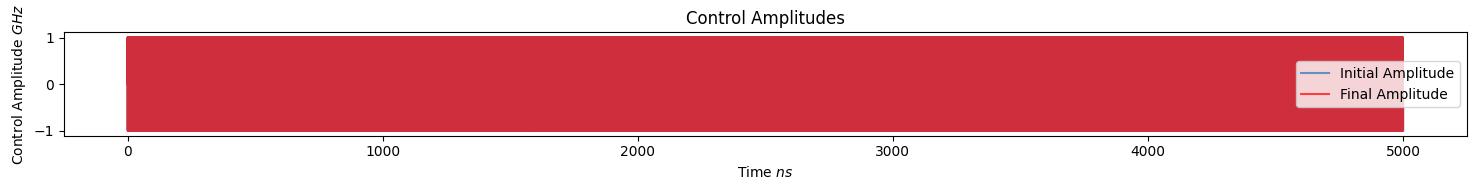
\includegraphics[width=0.95\linewidth]{vac2cat_effective_Hamiltonian_GRAPE_control1.png}
    \caption{vacuum to cat state control 1 pulse amplitudes}
    \label{fig:vac2cat_effective_Hamiltonian_GRAPE_control1}
\end{figure}
\begin{figure}[H]
    \centering
    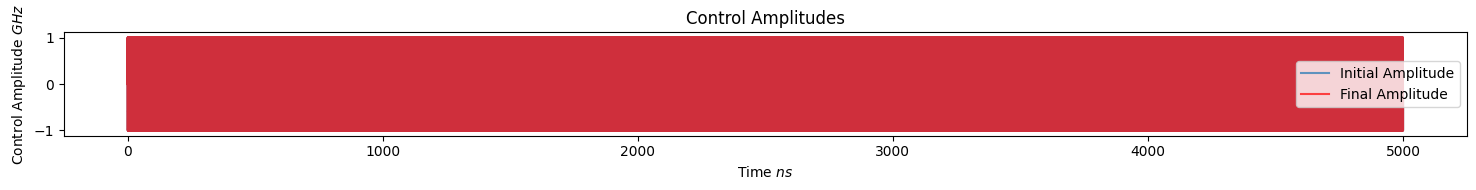
\includegraphics[width=0.95\linewidth]{vac2cat_effective_Hamiltonian_GRAPE_control2.png}
    \caption{vacuum to cat state control 2 pulse amplitudes}
    \label{fig:vac2cat_effective_Hamiltonian_GRAPE_control2}
\end{figure}
\begin{figure}[H]
    \centering
    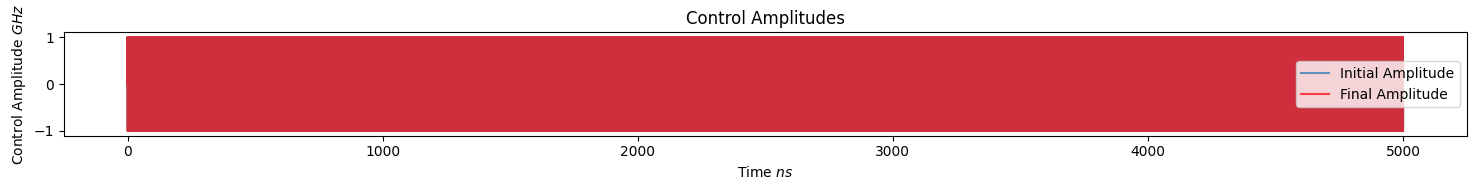
\includegraphics[width=0.95\linewidth]{vac2cat_effective_Hamiltonian_GRAPE_control3.png}
    \caption{vacuum to cat state control 3 pulse amplitudes}
    \label{fig:vac2cat_effective_Hamiltonian_GRAPE_control3}
\end{figure}

Forward simulation is given below to ensure that pulse optimization has run properly. 
\par
Simulation gives: 
\begin{itemize}
    \item sesolve final fidelity:  0.4390558062780975
    \item cavity ptrace fidelity:  0.44320315443027297
    \item qubit ptrace fidelity:  0.9871678390509413
    \item self-implemented final fidelity:  0.9529111010142354
\end{itemize}
\begin{figure}[H]
    \centering
    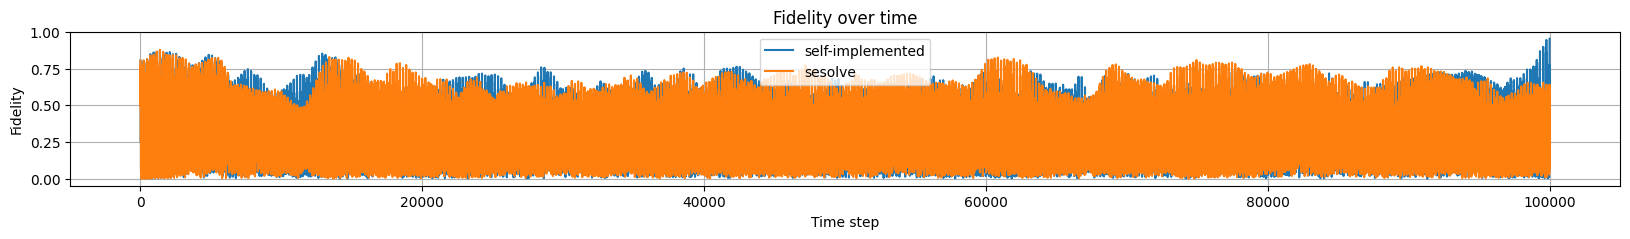
\includegraphics[width=0.95\linewidth]{vac2cat_effective_Hamiltonian_GRAPE_simulations.png}
    \caption{vacuum to cat state forward simulation}
    \label{fig:vac2cat_effective_Hamiltonian_GRAPE_simulations}
\end{figure}

It can be seen that the optimization results are not very satisfactory. 
Many tunings were attempted but none gave satisfactory results.
\par
At this point, we turned to look at a new python quantum control optimziation library, Krotov which builds on top of QuTip,
to see whether it can give better optimization results. Krotov’s optimization method is a gradient-based optimization algorithm like GRAPE. 
Krotov’s method distinguishes itself by guaranteeing monotonic convergence for near-continuous control fields. 
Besides the difference in optimization algorithm used, the Krotov package has the following incentives to be tried: 
\begin{itemize}
    \item Krotov is much better implemented than QuTip. For instance, Krotov allows display of optimization progress for every iteration. 
    \item Krotov allows inbuilds better customizability than QuTip. 
            For instance, Krotov allows for the optimization of the fidelity to be optimized.
\end{itemize}

Besides switching from QuTip to Krotov, the Hamiltonians are also redefined to be an interaction picture. 
The drift Hamiltonian ($H_0$) and control Hamiltonians ($H_1$, $H_2$, $H_3$) are defined as follows:

1. \textbf{Drift Hamiltonian} ($H_0$):
\begin{equation}
H_0 = \hbar \omega_r a^\dagger a + \frac{E_s}{2} \sigma_z + \frac{E_m}{2} \tau_z - \chi_m \tau_z \left(a^\dagger a + \frac{1}{2}\right) - \chi_s \sigma_z \left(a^\dagger a + \frac{1}{2}\right) - \frac{\chi_0}{2} \sigma_z \tau_z,
\end{equation}
where $\omega_r$ is the resonator frequency, $a$ and $a^\dagger$ are the annihilation and creation operators of the cavity, $E_s$ and $E_m$ are the energy levels of the qubit and the molecular orbital, $\sigma_z$ and $\tau_z$ are the Pauli Z operators for the qubit and the molecular orbital, respectively, and $\chi_m$, $\chi_s$, and $\chi_0$ are the dispersive shifts.

2. \textbf{Control Hamiltonians}:
   - $H_1$: This control Hamiltonian corresponds to the real part of the cavity drive. It is given by
     \begin{equation}
     H_1 = \left(a + a^\dagger\right),
     \end{equation}
     where $a$ and $a^\dagger$ are the annihilation and creation operators of the cavity.

   - $H_2$: This control Hamiltonian corresponds to the imaginary part of the cavity drive. It is given by
     \begin{equation}
     H_2 = -i\left(a - a^\dagger\right),
     \end{equation}
     where $a$ and $a^\dagger$ are the annihilation and creation operators of the cavity.

   - $H_3$: This control Hamiltonian corresponds to the drive on the qubit. It is given by
     \begin{equation}
     H_3 = \sigma_x,
     \end{equation}
     where $\sigma_x$ is the Pauli X operator for the qubit.
\\
The optimized results are as follow. 
\begin{figure}[H]
    \centering
    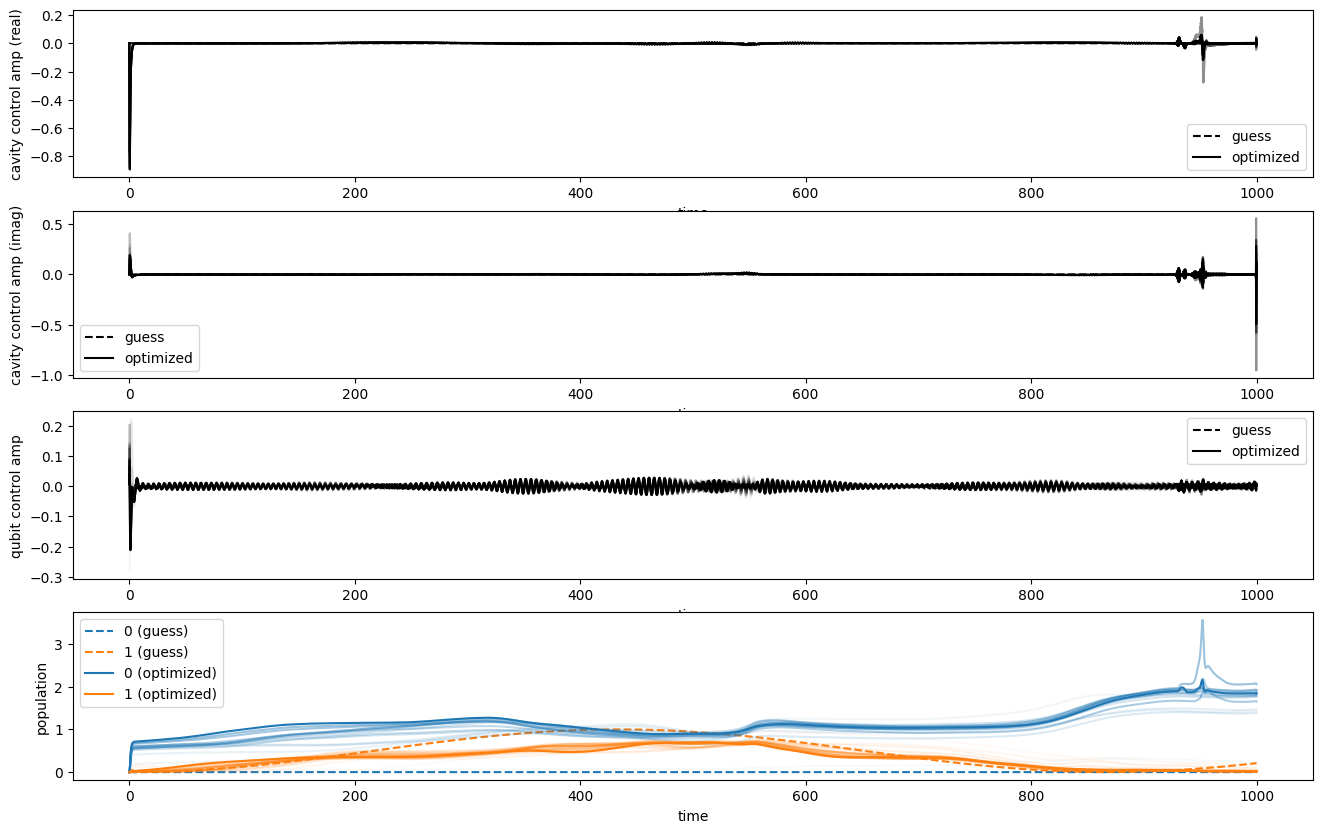
\includegraphics[width=0.95\linewidth]{vac2cat_krotov.png}
    \caption{
        (1st,2nd) The optimized control fields for the cavity drive (real and imaginary parts) and the qubit drive. \\
        (3rd) qubit control \\
        (4th) qubit population
    }
    \label{fig:vac2cat_krotov}
\end{figure}

Forward simulation is given below to ensure that pulse optimization has run properly. 
\\
Simulation gives: 
\begin{itemize}
    \item final fidelity:  0.9992259750482354
\end{itemize}

\begin{figure}[H]
    \centering
    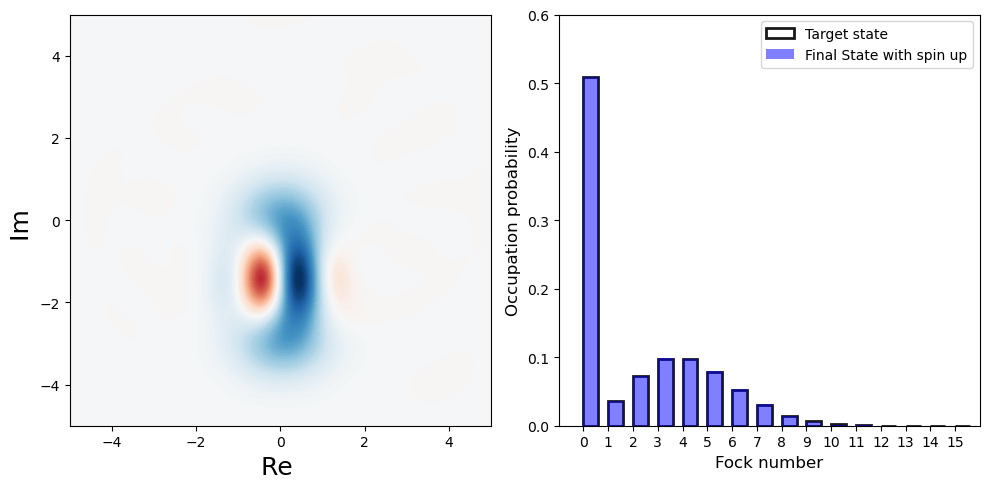
\includegraphics[width=0.95\linewidth]{vac2cat_simulation.png}
    \caption{
       (left) Wigner function representation of target cavity state and final cavity state 
       \\
       (right) target cavity state and final cavity state in Fock state basis
    }
    \label{fig:vac2cat_simulation}
\end{figure}

%%%%%%%%%%%%%%%%%%%%%%%%%%%%%%%
\section{Further Discussions}\label{sec:further_discussions}

There are a few points to be made regrading choosing the time parameters for optimization, evolution time (evo\_time) and number of time slices (n\_ts).
Evolution time (evo\_time), or equivalently the pulse length, can be estimated %TODO: ask chiyuan how is this calculated
Number of time slices (n\_ts) that is too small will lead to large error. 
n\_ts that is too large will result in long computation time; and also lead to fast oscillations in optimized pulses when optimization is using GRAPE.
Hence an appropriate n\_ts value needs to be tested via trial and error.
\par
It is unfortunate that there was not enough time to reach the initial goal of the project due to programming issues regrading QuTip and some other unexpected complications.
Firstly, it is understood that optimization should have been run with the fidelity of the cavity state alone, i.e. partial tracing out the qubit state when calculating fidelity. 
However, implementation of QuTip doesn't make this task easily achievable. QuTip doesn't calculate the fidelity of the current final state evolved from the current optimized pulse for each optimization iteration. 
Instead, it has a caching system that tries to minimize redundant calculations as the forward simulation process is very computation intensive due to the many matrix multiplications involved (which is proportional to number of time slices and the cavity state space truncation $N$).
As such, to implement partial trace fidelity for optimization using QuTip, one effectively needs to rewrite the bulk of the optimization code up to calling scipy optimization function. 
Attempt was made in this direction but was given up half way due to project time constraint. 
Besides, it was latered discovered that the Krotov package, a package based on top of QuTip, implements the optimziation process different from QuTip in such a was that allows for customization of fidelity. 
See How-to chapter, "How to define a new optimization functional" in Krotov documentation for details.
However, this was not attempted due to time constraint.
\par
Secondly, the project did not yet get to consider all physical constraints on the control pulses as discussed in chapter \ref{sec:pulse_constraints}.
The only constraint that was considered was the pulse amplitude constraint. To incorporate more physical constraints into pulse optimization, CRAB algorithm 
could be used which allows for the incorporation of physical constraints into the optimization process. Moreover, CRAB optimizes for functional basis coefficients 
rather than time-slice amplitudes of control pulses. This allos for arbitrary smoothness of the physical control pulses.
However, running CRAB requires more trial and error with choosing optimzation time parameters and functional basis parameters. 
From experience, GRAPE behaves much robustly in the QuTip implementation. One idea is to first run CRAB, aiming for a $~90\%$ fidelity and pass this optimized pulse into GRAPE for further optimizaiton. 
This is because CRAB usually runs faster than GRAPE, with only a small number of coefficients to be optimized. However, CRAB also has a smaller optimization landscap, making GRAPE a better choice for finer fidelity optimization. 
\par
Thirdly, one issue that was realised at the end was that the native oscillation frequency of the cavity seems to be causing the fast oscillations in the optimized pulses as seen in Fig \ref{fig:vac2cat_krotov}.
One idea was to transform the Hamiltonian to the rotating frame at the native oscillation frequency of the cavity to alleviate this issue. 
However, going to the rotating frame tags a rotating phase factor to the annihilation and creation operators of the cavity. 
As QuTip and Krotov only optimizes for real control pulses, so far in the control Hamiltonians that I used, control signal on the cavity has been separated into real and imaginary parts. 
With different rotating phase factors taged to the annihilation and creation operators of the cavity, the real and imaginary parts of the control pulses cannot be separated any more. 
This issue was not further looked into due to time constraint. 
\par
With more time, all three above stated problems should be solvable. All three problems come from technical programming issues. 
With these settled, the next step would be to use the final optimized control pulses to simulate the evolution of the original full Hamiltonian and compare the state fidelity. 
This is to check whether the optimized pulses violate the constraints for the effective Hamiltonian to be valid. 
Although the above three issues were not settled, this task of checking with the full Hamiltonian was still attempted. (the same code as the Krotov code)
However, the computation couldn't be completed in any reasonable amount of time. 
One idea is to make use of packages such as TensorFlow and CuPy to speed up matrix multiplications by through GPU acceleration.
This idea was attempted but also dropped half way due to time constraints. 
Besides, this idea didn't seem promising as it seemed that even with GPU acceleration, the computation time would still be unreasonable. 
If this task is completed and a fidelity generated. A good fidelity will signify that the control pulse is within the valid limits of the effective Hamiltonian. 
If the fidelity is not good, more constraints need to be added during pulse optimization. 
\par
Beyond state preparation for a close quantum system, the next step would be to consdier state preparation in an open and noisy system. 
Apart from switching from the Schrödinger equation to the Lindblad master equation or Liouville-von Neumann equation, this is a very similar optimization process. 
\par
Beoyond state preparations in close or open systems, a related next task would be to do control pulse optimizations for unitary gates, often called gate design.
Both single-mode and multi-mode gates can be potential targets. Though many of the optimization lessons learned and implemented in this project can be re-used for such a purpose, this project did not have the time to reach this point. 

\chapter{Conclusion}
In conclusion, this report explored quantum optimal control for state preparation in a cavity-coupled double quantum dot system. 
Pulse optimization was successfully performed using the effective Hamiltonian to achieve high fidelity state transfers, demonstrating the potential of numerical methods for designing control protocols. 
However, challenges arose when applying the optimized pulses to the full physical Hamiltonian, indicating the need for further refinement of the optimization process and the inclusion of additional physical constraints. 
Future work should focus on improving computational efficiency, incorporating open quantum system dynamics, and extending the techniques to gate design for quantum computing applications.

\appendix
\chapter{Sample Code} \label{sec:sample_code}
\lstinputlisting[
    language=Python, 
    linewidth=0.9\textwidth, 
    basicstyle=\small\ttfamily, 
    breaklines=true, 
    breakatwhitespace=true, 
    caption = selective spin flip optimization code, 
    label=code:selective_spin_flip]{selective_spin_flip.py}

\printbibliography
\end{document}